\documentclass[fleqn,10pt]{wlscirep}
\usepackage[utf8]{inputenc}
\usepackage[T1]{fontenc}
\usepackage{multirow}
\usepackage{tabularx}
\usepackage{booktabs}
\usepackage{float}
\usepackage{algorithm}
\usepackage{algorithmic}
\usepackage{amsthm}
\usepackage{xcolor}
\usepackage{url}
\captionsetup{font=small,labelfont={bf,rm},textfont=rm,justification=justified}
\newtheorem{proposition}{Proposition}

\renewcommand{\topfraction}{0.9}
\renewcommand{\bottomfraction}{0.8}
\renewcommand{\textfraction}{0.07}
\renewcommand{\floatpagefraction}{0.8}
\renewcommand{\dbltopfraction}{0.9}
\renewcommand{\dblfloatpagefraction}{0.8}
\setcounter{topnumber}{3}
\setcounter{bottomnumber}{2}
\setcounter{totalnumber}{4}
\setcounter{dbltopnumber}{3}

\newcommand{\Ltr}{\mathcal{L}^{\mathrm{tr}}}
\newcommand{\Lcv}{\mathcal{L}^{\mathrm{cv}}}
\newcommand{\Lte}{\mathcal{L}^{\mathrm{te}}}
\newcommand{\OGR}{\mathrm{OGR}}
\newcommand{\pmm}{$\pm$}

\title{OGR-Driven Dynamic Loss Balancing for Mitigating Gradient Starvation}

\author[1]{Lakshya}
\author[1,*]{Amit Kumar Bairwa}
\author[1,*]{Varun Tiwari}
\affil[1]{Department of Artificial Intelligence and Machine Learning, School of Computer Science and Engineering, Manipal University Jaipur, Jaipur--Ajmer Express Highway, Jaipur, India.}

\affil[*]{amitkumar.bairwa@jaipur.manipal.edu}
\affil[*]{varun.tiwari@jaipur.manipal.edu}
\affil[*]{Corresponding Authors}

\begin{abstract}
Jointly trained multimodal networks tend to rely on whichever modality is easiest to fit and leave the other encoders under-trained, a failure known as modality laziness or gradient starvation. We study a simple, generalization-aware remedy. First, we define the Overfitting-to-Generalization Ratio (OGR), the ratio of a modality's held-out loss to its training loss, as a scale-invariant per-modality diagnostic. Second, we propose MFC-A, a closed-loop controller that gives each unimodal auxiliary loss a weight proportional to a power of its inverse smoothed OGR, so that a modality that starts to memorise is throttled and the others are amplified within a fixed weight budget. MFC-A runs inside a single training run and needs no auxiliary networks, gradient surgery or noise injection. We compare it with eight baselines under one protocol (ten paired seeds; disjoint training, controller, tuning and test splits; paired significance tests) on two real audio--video benchmarks, AVE and CREMA-D (actor-disjoint), complemented by a controlled synthetic benchmark and a two-view control. On AVE, MFC-A maintains accuracy (80.2 vs.\ 79.9\%) while reducing the OGR gap by 63\% ($p{=}0.03$) and improving robustness to visual noise, blur and low light ($p<0.04$). On the synthetic benchmark it maintains accuracy while reducing the gap by 41\% ($p<0.001$). On CREMA-D, whose dominant modality is audio, it identifies the overfitting video stream correctly and maintains accuracy, but its gains are not significant. Confidence-based gradient modulation (OGM-GE) on AVE and offline Gradient Blending on CREMA-D achieve larger gains at the cost of a tuned hyper-parameter or an extra probe run. A follow-up variant that uses OGR to decide when to apply such modulation matches OGM-GE on AVE with a lower imbalance gap, but no variant is best on every dataset. The controller's arithmetic is negligible; its monitoring passes add 2--18\% wall-clock time.
\end{abstract}
\begin{document}

\flushbottom
\maketitle
\thispagestyle{empty}

\noindent\textbf{Keywords:} Multimodal learning, Modality imbalance, Gradient starvation, Dynamic loss balancing, Overfitting-to-Generalization Ratio (OGR), Audio--visual emotion recognition.

\section*{Introduction}
Multimodal models combine complementary signals, such as images, audio and text, and large unified architectures including CLIP\cite{radford2021learning}, Flamingo\cite{alayrac2022flamingo}, ImageBind\cite{girdhar2023imagebind} and Meta-Transformer\cite{zhang2023meta} have made this the default design for perception systems. Training such models jointly is nevertheless fragile. When one modality is easier to fit than another, gradient descent reduces the joint loss mainly through the easier modality, and the encoder of the harder modality receives little useful gradient. This phenomenon has been called modality laziness, modality competition\cite{huang2022modality} or, following the analysis of Pezeshki et al.\cite{pezeshki2021gradient}, gradient starvation.

The effect is often invisible in clean-data accuracy, because the dominant modality alone is enough to reach a good score. It becomes visible when the dominant modality is degraded: a model whose second encoder never developed cannot fall back on it. For example, an autonomous vehicle that has learned to rely on its camera may ignore an audible siren in fog, and a clinical model that relies on images may be unable to use the accompanying report when a scan is corrupted.

Existing remedies fall into a few families\cite{xu2025balancebenchmark}. Gradient Blending\cite{wang2020makes} estimates per-modality loss weights from the overfitting behaviour of unimodal probe models and keeps them fixed. Gradient-modulation methods such as OGM-GE\cite{peng2022balanced} and AGM\cite{li2023boosting} measure how confidently or quickly each modality fits the training data and slow the dominant one down. Gradient-geometry methods such as PCGrad\cite{yu2020gradient} and MMPareto\cite{wei2024mmpareto} resolve conflicts between the gradients of different objectives. Uncertainty weighting\cite{kendall2018multi} learns loss weights from a homoscedastic noise model. With the exception of Gradient Blending, these signals are computed on the training data: they describe how fast a modality is being fitted, not whether that fit generalises. A large gradient norm or a high training confidence can reflect useful learning or memorisation, and training-set statistics alone cannot separate the two.

This paper studies whether a generalization-based signal, measured online and used in closed loop, is a practical alternative, and makes three contributions. The first is a diagnostic: we define the per-modality Overfitting-to-Generalization Ratio, $\OGR_m=\Lcv_m/\Ltr_m$, and show that, unlike the raw generalization gap, it is invariant to the scale of each modality's loss, so that modalities with very different loss magnitudes can be compared directly (Proposition~\ref{prop:scale}); OGR is a measurement and can be logged in any training run, independently of the controller. The second is a controller, MFC-A, a threshold-free control law that sets each unimodal loss weight to a smoothed, inverse-OGR share of a fixed budget, so that throttling the relatively overfitting modality and amplifying the other are two halves of the same law rather than separate heuristics; unlike Gradient Blending, the weights adapt during a single run and need no probe models, and unlike OGM-GE and MMPareto, the method operates only on scalar loss weights. The third is a controlled evaluation in which MFC-A is compared with eight baselines under one protocol, with ten paired seeds, disjoint training, controller-validation, tuning and test splits, identical architectures and optimisers, and paired significance tests. The experiments cover two real audio--video benchmarks, AVE\cite{tian2018audio} (vision-dominant) and CREMA-D\cite{cao2014crema} (audio-dominant, actor-disjoint split), together with a controlled synthetic benchmark and a two-view spectrogram control, and they include a component ablation, a sensitivity analysis, a capacity study, robustness to graded visual degradations, gradient-level evidence, a complete cost breakdown and the per-epoch traces of OGR and loss weights.
Our results are deliberately reported with their variance. MFC-A never reduces accuracy significantly, reduces the imbalance measured by OGR (significantly on AVE and on the synthetic benchmark), and improves robustness on AVE; it is not the strongest method on every dataset. We discuss when the method helps and when a simpler or offline alternative is preferable.

\section*{Related work}
\subsection*{Static and offline re-weighting}
Gradient Blending\cite{wang2020makes} showed that multimodal networks often underperform their best unimodal counterpart because they overfit, and derived blending weights proportional to the generalization gain divided by the squared growth of the overfitting gap, measured on unimodal and multimodal probe models. The weights are principled but are estimated from separate training runs and then fixed. Uncertainty weighting\cite{kendall2018multi} learns one log-variance per task; it was designed for multi-task regression and classification and tends to down-weight high-loss objectives, which in the multimodal setting is usually the starved modality. Focal-style losses\cite{lin2017focal} address class imbalance rather than modality imbalance.

\subsection*{Dynamic modulation}
OGM-GE\cite{peng2022balanced} computes, for every mini-batch, the ratio of the two modalities' training-set confidence for the correct class, scales down the encoder gradients of the more confident modality by $1-\tanh(\alpha(\rho-1))$, and adds Gaussian gradient noise to preserve generalization. GradNorm\cite{chen2018gradnorm} equalises per-task gradient norms relative to their training-loss ratios. PCGrad\cite{yu2020gradient} projects conflicting task gradients onto each other's normal planes. AGM\cite{li2023boosting} estimates each modality's contribution with a perturbation-based score and modulates its gradient. Multi-loss gradient modulation\cite{kontras2024improving} balances the magnitudes of several loss terms jointly, OLM\cite{zong2024balancing} modulates logits rather than gradients, and MMPareto\cite{wei2024mmpareto} combines multimodal and unimodal gradients with a Pareto (MGDA\cite{desideri2012mgda}) rule when they conflict. PMR\cite{xu2025balancebenchmark} uses class prototypes to re-balance learning, and MBPO\cite{liu2025modality} treats modality-specific hallucination as a preference-optimisation problem. AMSA\cite{wang2023amsa} applies adaptive loss modulation to multimodal sentiment analysis.

MFC-A differs from these methods in the signal it observes and in where it acts. It observes the ratio of held-out to training loss for each modality, a generalization signal, whereas OGM-GE, GradNorm and AGM observe training-set confidence, gradient norms or training-loss rates, and MMPareto observes gradient directions. It acts only on two scalar loss weights per epoch, with no per-batch gradient manipulation, no noise and no extra models. Gradient Blending is the closest in spirit, since it also uses overfitting behaviour; MFC-A can be viewed as an online, closed-loop, single-run counterpart of that principle. Table~\ref{tab:relwork} summarises the positioning.

\begin{table}[t]
\caption{\textbf{Positioning of MFC-A among imbalance-mitigation methods.} ``Signal'' is the quantity a method monitors; ``Generalization-aware'' indicates whether that signal involves held-out data.}
\label{tab:relwork}
\centering
\small
\begin{tabularx}{\linewidth}{@{}lXccl@{}}
\toprule
\textbf{Method} & \textbf{Signal} & \textbf{Online} & \textbf{Generalization-aware} & \textbf{Acts on} \\ \midrule
Gradient Blending\cite{wang2020makes} & Overfitting of probe models & No & Yes & Fixed loss weights \\
Uncertainty weighting\cite{kendall2018multi} & Learned noise variance & Yes & No & Loss weights \\
GradNorm\cite{chen2018gradnorm} & Gradient norms, training-loss rates & Yes & No & Loss weights \\
OGM-GE\cite{peng2022balanced} & Training confidence ratio & Yes & No & Encoder gradients + noise \\
MMPareto\cite{wei2024mmpareto} & Gradient conflict & Yes & No & Encoder gradients \\
\textbf{MFC-A (ours)} & Held-out/training loss ratio (OGR) & Yes & Yes & Loss weights \\ \bottomrule
\end{tabularx}
\end{table}

\subsection*{Multimodal fusion and visual representation}
Imbalance interacts with the fusion design. L3-Net\cite{arandjelovic2017look} learned audio--visual correspondence from unlabelled video, attention bottlenecks\cite{nagrani2021attention} force cross-modal exchange inside transformers, and recursive joint cross-modal attention\cite{praveen2024recursive} improves audio--visual emotion recognition without explicit loss re-weighting. Barra et al.\cite{barra2023multimodal} combine voice analysis and facial-expression recognition for emotion recognition on IEMOCAP, targeting assistive healthcare settings; audio--visual emotion recognition is also the task of our CREMA-D benchmark. On the audio side, acoustic images, i.e.\ spatially resolved spectra from a microphone array aligned with the camera, have been used as training-time privileged information: Sanguineti et al.\cite{sanguineti2020leveraging} distil them, through a self-supervised audio--visual correspondence task, into monaural audio networks that then outperform audio models trained without them on classification and cross-modal retrieval. Making such sensors portable is an active hardware problem: Greco\cite{greco2023feasibility} shows in simulation that an optimised 32-microphone array of about $20{\times}20$\,cm can match or exceed a 128-microphone, $50{\times}50$\,cm array below 4\,kHz. On the visual side, the strength of the pretrained backbone largely determines how dominant the visual stream becomes. In vision-only tasks the backbone has moved from CNNs to transformers; a survey of deep human pose estimation\cite{lan2023pose} documents this shift and identifies efficient models and multi-modal learning as open directions. The backbone choice itself is consequential: in deepfake image detection, for example, hybrids that pair a Swin transformer with CNN backbones (DenseNet, ConvNeXt, MobileNet) or with CLIP have been reported to outperform their standalone counterparts, with a ConvNeXt--Swin combination giving the highest accuracy\cite{mishra2026deepfake}; we hypothesise that this choice likewise affects how dominant the visual stream becomes in a multimodal model. We use a frozen ImageNet ResNet-18\cite{he2016deep} as a deliberately modest visual encoder: on AVE it yields the dominant stream, whereas on CREMA-D audio dominates, which lets us test MFC-A in both regimes. Loss-level balancing is complementary to all of these architectural choices.

\subsection*{Adaptive and evolutionary optimisation}
MFC-A adapts an optimisation hyper-parameter, the loss weights, during training, which places it within the broader study of adaptive optimisation. Lan et al.\cite{lan2022time} show that comparing optimisers by the number of function evaluations is misleading when their per-iteration overhead differs, and propose measuring efficiency as objective gain per unit of computation time, split into evaluation and overhead time. Following this, we report wall-clock time and FLOPs separately for the controller arithmetic, the monitoring passes and the method-specific work of every method (Table~\ref{tab:cost}). In a related spirit, Lan et al.\cite{lan2022class} evaluate class-binarization strategies for neuroevolution (NEAT) not only by accuracy but also by multiclass degradation, evolutionary efficiency and robustness; we likewise report accuracy, modality balance (OGR gap), training cost and robustness rather than accuracy alone. Unlike population-based approaches, MFC-A adapts a single run with a closed-form rule, so it has no population cost, but it also cannot explore the weight space globally.

\subsection*{Robustness under adverse visual conditions}
Robustness to corrupted inputs is usually evaluated with synthetic corruptions such as noise, blur and occlusion\cite{hendrycks2019benchmarking}. Generative augmentation goes further: SUSTechGAN\cite{lan2025sustechgan} synthesises rain and night driving images with attention-based multi-scale generators, and adding them to the training set improves YOLOv5 detection under those conditions. Augmentation and modality balancing tackle visual degradation from opposite directions: the former makes the visual encoder itself robust, whereas balancing keeps a second modality informative for when the visual encoder fails. We evaluate the latter under additive noise and three pixel-level degradations (blur, occlusion and low light).

\section*{Problem formulation}
We consider $M$ modalities indexed by $m\in\{1,\dots,M\}$; all experiments use $M{=}2$, written $v$ (``visual'' or first stream) and $a$ (``audio'' or second stream). A sample is $(\mathbf{x},y)$ with $\mathbf{x}=\{x^m\}_m$ and class label $y$. Each modality has an encoder $z_m=E_m(x^m;\theta_m)$ and a linear unimodal head $h_m$, and a fusion head $g$ acts on the concatenated embeddings (late fusion). We write
\begin{equation}
\mathcal{L}_{\mathrm{joint}} = \ell\big(g([z_v;z_a]),y\big), \qquad \mathcal{L}_m=\ell\big(h_m(z_m),y\big),
\end{equation}
where $\ell$ is the cross-entropy. All methods in this paper minimise
\begin{equation}
\mathcal{L}(t)=\mathcal{L}_{\mathrm{joint}}+\sum_{m}\lambda_m(t)\,\mathcal{L}_m ,
\label{eq:objective}
\end{equation}
and differ only in how $\lambda_m(t)$ is chosen (or, for OGM-GE and MMPareto, in how gradients are post-processed). The baseline uses $\lambda_m\equiv1$. Because $\mathcal{L}_{\mathrm{joint}}$ is not re-weighted, the weights redistribute the \emph{auxiliary} unimodal supervision that each encoder receives.

Gradient starvation arises when one encoder, say $E_v$, reduces $\mathcal{L}_{\mathrm{joint}}$ much faster than $E_a$. Once the fused prediction is confident, the gradient of $\mathcal{L}_{\mathrm{joint}}$ with respect to $\theta_a$ becomes small, and $E_a$ is left under-trained\cite{pezeshki2021gradient,huang2022modality}. The unimodal terms in Eq.~(\ref{eq:objective}) keep supplying gradient to each encoder, and their weights determine how strongly.

\paragraph{Data splits.} We use four disjoint subsets: $\mathcal{D}_{\mathrm{tr}}$ (training), $\mathcal{D}_{\mathrm{cv}}$ (controller validation, the only held-out data any controller may read), $\mathcal{D}_{\mathrm{tune}}$ (checkpoint and hyper-parameter selection) and $\mathcal{D}_{\mathrm{te}}$ (test, used once after training). For epoch $t$ we denote by $\Ltr_m(t)$ and $\Lcv_m(t)$ the mean loss of head $h_m$ over $\mathcal{D}_{\mathrm{tr}}$ and $\mathcal{D}_{\mathrm{cv}}$, evaluated in inference mode at the end of the epoch.

\section*{Method}
\subsection*{The Overfitting-to-Generalization Ratio}
The generalization gap of modality $m$ is
\begin{equation}
G_m(t)=\Lcv_m(t)-\Ltr_m(t).
\label{eq:gap}
\end{equation}
We define the Overfitting-to-Generalization Ratio as
\begin{equation}
\OGR_m(t)=\frac{\Lcv_m(t)}{\Ltr_m(t)+\epsilon}=1+\frac{G_m(t)}{\Ltr_m(t)+\epsilon},
\label{eq:ogr}
\end{equation}
with $\epsilon=10^{-8}$. $\OGR_m\approx1$ means that what modality $m$ has learned transfers to held-out data; $\OGR_m\gg1$ means that its training loss keeps falling without a matching fall in held-out loss, that is, it is memorising. Equivalently, $\log\OGR_m=\log\Lcv_m-\log\Ltr_m$ is the generalization gap measured in log-loss.

\begin{proposition}[Scale invariance]
\label{prop:scale}
Let $\Ltr_m$ and $\Lcv_m$ be multiplied by a common factor $c>0$ (for instance by a change of loss normalisation, label smoothing or temperature that rescales the loss of head $h_m$). Then $\OGR_m$ is unchanged (up to $\epsilon$), whereas $G_m$ is multiplied by $c$.
\end{proposition}
\begin{proof}
$c\Lcv_m/(c\Ltr_m)=\Lcv_m/\Ltr_m$ and $c\Lcv_m-c\Ltr_m=c\,G_m$.
\end{proof}

Proposition~\ref{prop:scale} matters because the two heads of an imbalanced model operate at very different loss levels. In our synthetic benchmark, after 20 epochs the visual head has $\Ltr_v\approx0.15$ and the audio head $\Ltr_a\approx1.55$ (Fig.~\ref{fig:dyn_syn}). An identical raw gap of $0.3$ then means that the visual head's held-out loss is three times its training loss, while the audio head's is only 19\% above it. The raw gap ranks the two modalities as equally overfitting, whereas OGR identifies the visual head as the one that is memorising. We also test this empirically by replacing OGR with the raw gap inside the controller (signal ablation, Table~\ref{tab:ablation}).

\subsection*{MFC-A: inverse-OGR closed-loop weighting}
MFC-A updates the weights once per epoch from smoothed OGRs. Let $\mathcal{W}_t=\{\max(1,t-W+1),\dots,t\}$ be a window of the last $W$ epochs. The windowed ratio is
\begin{equation}
\widetilde{\OGR}_m(t)=\frac{\frac{1}{|\mathcal{W}_t|}\sum_{k\in\mathcal{W}_t}\Lcv_m(k)}{\frac{1}{|\mathcal{W}_t|}\sum_{k\in\mathcal{W}_t}\Ltr_m(k)+\epsilon}.
\label{eq:window}
\end{equation}
Each modality receives a target weight equal to its share of the inverse OGRs raised to a control strength $\gamma>0$, scaled so that the targets sum to $M$:
\begin{equation}
\pi_m(t)=\frac{M\,\widetilde{\OGR}_m(t)^{-\gamma}}{\sum_{k=1}^{M}\widetilde{\OGR}_k(t)^{-\gamma}}.
\label{eq:target}
\end{equation}
For $t<T_w$ (warm-up) all weights stay at 1. Afterwards the weights follow the targets through an exponential moving average and are clipped:
\begin{equation}
\lambda_m(t+1)=\operatorname{clip}\!\big(\beta\,\lambda_m(t)+(1-\beta)\,\pi_m(t),\;\lambda_{\min},\;\lambda_{\max}\big).
\label{eq:update}
\end{equation}
\paragraph{Properties.} (i) If all modalities generalise equally ($\widetilde{\OGR}_m$ equal), then $\pi_m=1$ and MFC-A reduces to the baseline. (ii) Because $\sum_m\pi_m=M$ and $\lambda_m(0)=1$, induction on Eq.~(\ref{eq:update}) gives $\sum_m\lambda_m(t)=M$ whenever clipping is inactive, so MFC-A redistributes a fixed budget of auxiliary supervision rather than changing the overall loss scale. (iii) A modality with above-average OGR receives $\pi_m<1$ (it is \emph{throttled}), and the others receive $\pi_m>1$ (they are \emph{amplified}); the two ``rules'' of our first description are therefore the two sides of Eq.~(\ref{eq:target}). (iv) The update has no thresholds. $\gamma$ sets how sharply the budget is moved towards the better-generalising modality ($\gamma\to0$ recovers the baseline); $W$, $\beta$, $T_w$ and $[\lambda_{\min},\lambda_{\max}]$ only control smoothing, start time and safety bounds, and we show below that results are insensitive to them.

\paragraph{Selecting $\gamma$ without test data.} The aim of balancing is to reduce imbalance \emph{while maintaining accuracy}. We therefore fix the following rule in advance: among $\gamma\in\{1,2,3\}$, choose the value with the smallest OGR gap on the controller split $\mathcal{D}_{\mathrm{cv}}$ (at the selected checkpoint), subject to its mean accuracy on $\mathcal{D}_{\mathrm{tune}}$ being within 0.5 points of the baseline's. The rule uses only $\mathcal{D}_{\mathrm{cv}}$ and $\mathcal{D}_{\mathrm{tune}}$, never $\mathcal{D}_{\mathrm{te}}$. Results for every $\gamma$ are reported as well (Table~\ref{tab:sens}). Gradient Blending's offline weights\cite{wang2020makes} use a different functional form, namely generalization gain divided by the squared overfitting growth.

\begin{algorithm}[t]
\caption{MFC-A (the method evaluated in all main experiments)}
\label{alg:mfca}
\begin{algorithmic}[1]
\STATE \textbf{Input:} control strength $\gamma$, window $W$, EMA factor $\beta$, warm-up $T_w$, bounds $[\lambda_{\min},\lambda_{\max}]$, splits $\mathcal{D}_{\mathrm{tr}},\mathcal{D}_{\mathrm{cv}}$
\STATE $\lambda_m\leftarrow1$ and history $H_m\leftarrow\emptyset$ for all $m$
\FOR{epoch $t=0,\dots,T-1$}
  \FOR{each mini-batch $B\subset\mathcal{D}_{\mathrm{tr}}$}
    \STATE update $\theta$ with one SGD step on $\mathcal{L}_{\mathrm{joint}}+\sum_m\lambda_m\mathcal{L}_m$ \hfill Eq.~(\ref{eq:objective})
  \ENDFOR
  \FOR{each modality $m$}
    \STATE $\Ltr_m\leftarrow$ mean loss of $h_m$ on $\mathcal{D}_{\mathrm{tr}}$; \; $\Lcv_m\leftarrow$ mean loss of $h_m$ on $\mathcal{D}_{\mathrm{cv}}$ \hfill (inference mode)
    \STATE append $(\Ltr_m,\Lcv_m)$ to $H_m$; \; compute $\widetilde{\OGR}_m$ from the last $W$ entries \hfill Eq.~(\ref{eq:window})
  \ENDFOR
  \IF{$t\ge T_w$}
    \FOR{each modality $m$}
      \STATE $\pi_m\leftarrow M\,\widetilde{\OGR}_m^{-\gamma}/\sum_k\widetilde{\OGR}_k^{-\gamma}$ \hfill Eq.~(\ref{eq:target})
      \STATE $\lambda_m\leftarrow\operatorname{clip}(\beta\lambda_m+(1-\beta)\pi_m,\lambda_{\min},\lambda_{\max})$ \hfill Eq.~(\ref{eq:update})
    \ENDFOR
  \ENDIF
  \STATE keep the checkpoint with the best accuracy on $\mathcal{D}_{\mathrm{tune}}$
\ENDFOR
\end{algorithmic}
\end{algorithm}

\paragraph{Variant without the extra training pass.} Line 8 evaluates the training loss with an additional inference pass over $\mathcal{D}_{\mathrm{tr}}$. A cheaper variant, ``MFC-A (running)'', instead uses the average of the mini-batch losses already computed during the epoch. These are measured in training mode and are therefore slightly biased, but they remove the extra pass (see the cost analysis).

\paragraph{Threshold variant (MFC-T).} The first version of this work described a threshold controller: it multiplies $\lambda_m$ by $0.95$ when $\widetilde{\OGR}_m>\tau_{\mathrm{hi}}{=}1.2$, multiplies it by $1.05$ when $\widetilde{\OGR}_m<\tau_{\mathrm{lo}}{=}1.05$ and $\Ltr_m>0.5$, and clips it to $[0.1,5]$. We keep it as a separate baseline, labelled MFC-T. \emph{Every result labelled MFC-A uses Algorithm~\ref{alg:mfca}.}

\subsection*{Cost and complexity}
Let $F$ be the forward cost of the model per sample, so that one training step costs approximately $3F$ per sample (forward and backward), and let $N_{\mathrm{tr}},N_{\mathrm{cv}},N_{\mathrm{tune}}$ be the split sizes and $T$ the number of epochs. Standard training with per-epoch checkpoint selection costs $T(3FN_{\mathrm{tr}}+FN_{\mathrm{tune}})$. MFC-A adds three costs. Its monitoring requires two inference passes per epoch, costing $T\,F\,(N_{\mathrm{tr}}+N_{\mathrm{cv}})$ in total ($T\,F\,N_{\mathrm{cv}}$ for the running variant). Its controller arithmetic needs $O(MW)$ scalar operations per epoch ($4W{+}12$ for $M{=}2$), that is, $O(TMW)$ in total. Its memory overhead is $O(MW)$ scalars in addition to the $O(|\theta|)$ model parameters.
The total time complexity is therefore $O\big(TF(N_{\mathrm{tr}}+N_{\mathrm{cv}}+N_{\mathrm{tune}})\big)$, of the same order as standard training but with a larger constant. The first version of this paper reported ``zero additional FLOPs'' while counting only the controller arithmetic. That statement was incomplete, and we now report all three components separately (Table~\ref{tab:cost}).

\section*{Experimental setup}
\subsection*{Datasets}
\paragraph{Synthetic benchmark.} To control the degree of imbalance we generate a six-class problem with scikit-learn's \texttt{make\_classification} (6,000 samples, 96 features of which 48 are informative and 12 redundant, one cluster per class, class separation 0.6, 5\% label noise, \texttt{random\_state}=42). After standardisation, the first 64 features plus Gaussian noise with standard deviation 0.2 form the first stream (``visual-like'', easy), and the remaining 32 features plus Gaussian noise with standard deviation 0.9 form the second stream (``audio-like'', hard). Both streams describe the same sample and share its label by construction, so no cross-dataset pairing is involved. This benchmark contains no images or audio; it isolates the optimisation phenomenon under a known, strong imbalance.

\paragraph{CREMA-D audio--video (main real-data benchmark).} CREMA-D\cite{cao2014crema} contains audio--visual recordings of 91 actors speaking 12 sentences with six emotions (anger, disgust, fear, happiness, neutral, sadness). Each clip provides both modalities, so the pairing and the label (the clip's emotion) are given by the recording itself. We use the 7,439 clips that are available in both the original 16-kHz audio release and a public face-cropped video release with 16 frames per clip at $224{\times}224$. \emph{Audio:} a 64-band log-mel spectrogram (25-ms window, 10-ms hop, 512-point FFT) summarised by the per-band mean and standard deviation of the log-mel values and of their temporal deltas (256 dimensions). \emph{Video:} eight evenly spaced frames encoded by a frozen ImageNet ResNet-18\cite{he2016deep} and averaged (512 dimensions). Audio and video are therefore synchronised at the clip level. Splits are made by actor, so that no speaker appears in more than one split (about 55/13/9/14 actors and 4,490/1,065/736/1,148 clips for seed 0). In this dataset audio is the stronger modality (a logistic-regression probe reaches 41\% with audio and 33\% with video on held-out actors, against 16.7\% chance), so the controller must identify the dominant modality from the data rather than assume it.

\paragraph{AVE audio--video events (second real-data benchmark).} The Audio-Visual Event dataset\cite{tian2018audio} contains 4,143 ten-second YouTube clips annotated with one of 28 event categories (for example church bell, barking dog, violin, race car), each with sound and video from the same recording. It is a standard benchmark in the modality-imbalance literature\cite{peng2022balanced,li2023boosting,wei2024mmpareto}. We use the original release and its official train/validation/test lists. The official test list (402 clips) is the fixed test set $\mathcal{D}_{\mathrm{te}}$ for every seed; the official training and validation clips are re-split per seed, by YouTube video ID, into $\mathcal{D}_{\mathrm{tr}}/\mathcal{D}_{\mathrm{cv}}/\mathcal{D}_{\mathrm{tune}}$ (75/15/10\%), and clips whose video ID also appears in the test list are removed from training. \emph{Video:} eight frames sampled evenly over the clip (shorter side 256, centre crop 224) and encoded by the same frozen ResNet-18 (512 dimensions). \emph{Audio:} the same 256-dimensional log-mel statistics as for CREMA-D, computed from the 16-kHz mono soundtrack. The same pixel-level degradations are applied for robustness testing.

\paragraph{CREMA-D spectrogram views (control).} For continuity with the first submission we keep its second experiment, in which two feature views are computed from the same mel-spectrogram image: a 64-dimensional PCA of the $224{\times}224$ image (fitted on a fixed 60\% subset) and 48 per-band statistics (mean, standard deviation and maximum over 16 mel bands). These views come from one underlying signal and are \emph{not} two modalities, so we use them only as a feature-view control. The public copy of these images carries no file names, so actor-disjoint splitting is not possible and samples are split at random (stratified by construction).

\paragraph{Dataset statistics and an example instance.} Table~\ref{tab:datasets} summarises the four datasets. As an example of one paired training instance from CREMA-D: clip \texttt{1001\_DFA\_ANG\_XX} (actor 1001 saying ``Don't forget a jacket'' with anger) yields a 512-dimensional video vector (eight face frames through ResNet-18, averaged) and a 256-dimensional audio vector (log-mel statistics of the same recording), and its label is \emph{anger}; because the split is by actor, all 82 clips of actor 1001 fall into the same split. For AVE, clip \texttt{c---zaDCTaE} yields the same two vectors from its own frames and soundtrack, with label \emph{church bell}. No sample of one dataset is ever combined with a sample of another.

\begin{table}[t]
\caption{\textbf{Dataset statistics.} Per-class counts are given as the full list (six classes) or as min--max (AVE, 28 classes). Splits: train/controller/tune/test.}
\label{tab:datasets}
\centering
\footnotesize
\setlength{\tabcolsep}{3pt}
\begin{tabularx}{\linewidth}{@{}lXccl@{}}
\toprule
\textbf{Dataset} & \textbf{Streams (pairing)} & \textbf{Samples} & \textbf{Classes} & \textbf{Per-class counts / split rule} \\ \midrule
CREMA-D audio--video & face video + audio of the same clip & 7,439 (91 actors) & 6 & 1271/1271/1270/1271/1087/1269; 60/15/10/15\% by actor \\
AVE & video + soundtrack of the same clip & 4,134 & 28 & 60--188 (test: 6--18); official test (402), rest 75/15/10\% by video ID \\
Synthetic & two noisy views of one generated vector & 6,000 & 6 & 991--1012; 60/15/10/15\% by sample \\
Spectrogram views & two features of one spectrogram & 7,442 & 6 & 1271 (neutral: 1087); 60/15/10/15\% by sample \\ \bottomrule
\end{tabularx}
\end{table}

\subsection*{Models and training}
Each stream is encoded by a two-layer MLP (Linear--ReLU--Dropout--Linear--ReLU) followed by a linear unimodal head; a linear fusion head acts on the concatenated embeddings. Hidden and embedding widths (first stream / second stream / embedding) are 128/64/32 for the synthetic benchmark (17,426 parameters), 256/128/64 for CREMA-D audio--video and AVE (190,482 and 196,180 parameters) and 128/64/64 for the spectrogram control (25,426 parameters). Dropout is 0.3 (0.4 for the synthetic second stream). All methods use SGD with learning rate 0.01, momentum 0.9, weight decay $5{\times}10^{-4}$ and batch size 64, for 30 epochs (synthetic) or 40 epochs (real data). Features are standardised with training-split statistics. The splits are 60/15/10/15\% for $\mathcal{D}_{\mathrm{tr}}/\mathcal{D}_{\mathrm{cv}}/\mathcal{D}_{\mathrm{tune}}/\mathcal{D}_{\mathrm{te}}$, except on AVE, where the official test list is kept (2,798/560/374/402 clips for seed 0). Each seed (0--9) fixes the split, the initialisation and the mini-batch order, and the same seed is used for every method, so all comparisons are paired.

\subsection*{Baselines}
All baselines are implemented in the same code base with the architecture, objective (Eq.~\ref{eq:objective}), optimiser, splits and seeds described above. The \textbf{Baseline} uses $\lambda_v{=}\lambda_a{=}1$. For \textbf{Gradient Blending}\cite{wang2020makes}, a unimodal probe is trained for six epochs; between probe epochs 2 and 6 we measure on $\mathcal{D}_{\mathrm{cv}}$ the generalization gain $G_m$ (drop in held-out loss) and the overfitting growth $O_m$ (growth of the gap), and set fixed weights $\lambda_m\propto G_m/O_m^2$, normalised to sum to 2, with the probe cost charged to the method. \textbf{Uncertainty weighting}\cite{kendall2018multi} minimises $\mathcal{L}_{\mathrm{joint}}+\sum_m(e^{-s_m}\mathcal{L}_m+s_m)$ with learned $s_m$. For \textbf{MMPareto}\cite{wei2024mmpareto}, the gradients of $\mathcal{L}_{\mathrm{joint}}$ and of $\mathcal{L}_m$ for each encoder are averaged when their cosine similarity is non-negative and otherwise combined with the two-task MGDA min-norm weights, and the result is rescaled to the norm of their sum. For \textbf{OGM-GE}\cite{peng2022balanced}, the confidence ratio $\rho$ is computed per mini-batch from the fusion-head logits split by modality, the encoder gradients of the more confident modality are scaled by $1-\tanh(\alpha(\rho-1))$, and Gaussian gradient enhancement with the per-tensor gradient standard deviation is applied; $\alpha\in\{0.1,0.3,0.8\}$ is selected per dataset on $\mathcal{D}_{\mathrm{tune}}$. We also re-implemented three recent modality-balancing methods. \textbf{AGM}\cite{li2023boosting} estimates each modality's contribution from the responses of the fused model with one modality masked and modulates the gradient entering the fusion layer from each encoder by the resulting discrepancy (with the exponent capped as in the authors' code); $\alpha\in\{0.1,0.5,1.0\}$. \textbf{PMR}\cite{fan2023pmr} builds per-modality class prototypes from a fixed tenth of the training set, adds a prototypical cross-entropy weighted by a continuous imbalance coefficient to accelerate the slower modality, and applies a prototypical entropy regulariser to the dominant modality during the first quarter of training; $\alpha\in\{1,2\}$ and $\mu\in\{10^{-3},10^{-2}\}$, the values stated in the paper. \textbf{OLM}\cite{zong2024balancing} learns online weights for the two modality shares of the fused logits during training, driven by the unimodal losses on $\mathcal{D}_{\mathrm{cv}}$ (late-fusion variant, without the transformer fusion block; because the published loss is minimised by all-zero weights, we normalise it to preserve the total magnitude and clamp the weights to $[0.1,10]$); $\eta\in\{0.01,0.1,1\}$. All three use the shared objective and have their hyper-parameters selected on $\mathcal{D}_{\mathrm{tune}}$; every deviation from the original papers is documented in the released code. \textbf{MFC-T} is the threshold variant described above.
MFC-A uses $W{=}5$, $\beta{=}0.7$, $T_w{=}3$ and $[\lambda_{\min},\lambda_{\max}]=[0.2,1.8]$ on all datasets; these values were fixed before the present experiments. $\gamma$ is chosen per dataset by the rule above, which yields $\gamma{=}3$ (AVE), $\gamma{=}2$ (CREMA-D audio--video), $\gamma{=}3$ (synthetic) and $\gamma{=}2$ (spectrogram views). The plain law ($\gamma{=}1$) is reported in every table as well.

\subsection*{Metrics and statistics}
We report, on $\mathcal{D}_{\mathrm{te}}$ at the checkpoint selected on $\mathcal{D}_{\mathrm{tune}}$: the accuracy of the fused prediction; the accuracy of each unimodal head (a direct measure of how well each encoder was trained); the \emph{OGR gap} $|\OGR^{\mathrm{te}}_v-\OGR^{\mathrm{te}}_a|$ with $\OGR^{\mathrm{te}}_m=\Lte_m/\Ltr_m$ (lower means more balanced); and robustness, namely accuracy when zero-mean Gaussian noise with standard deviation $\sigma\in\{0.5,1,2,3\}$ is added to the standardised first-stream features. For the two real audio--video datasets we also degrade the raw video frames before encoding (Gaussian blur with kernel 21 and $\sigma{=}6$; a $112{\times}112$ black occluder at a random position; low light, i.e.\ brightness $\times0.25$ plus sensor noise with standard deviation $0.05$) and evaluate a missing-video condition. All numbers are mean $\pm$ standard deviation over ten seeds. Differences from MFC-A are tested with a two-sided paired $t$-test over seeds\cite{bouthillier2021accounting}; $^{*}$ marks $p<0.05$. We do not correct for multiple comparisons, so isolated $p$-values near 0.05 should be read with caution. The per-epoch logs of every run, including $\lambda_m(t)$, $\OGR_m(t)$ and all split losses, are released with the code.

\section*{Results}
\subsection*{Main comparison}
Tables~\ref{tab:main_av}--\ref{tab:main_spec} report the main results, real-data benchmarks first.

\emph{AVE (Table~\ref{tab:main_ave}).} AVE is vision-dominant: the video head reaches about 74\% and the audio head about 49\%, and in the baseline the video OGR grows to about 41 while the audio OGR stays near 2. MFC-A ($\gamma{=}3$) throttles the video auxiliary loss to its lower bound and amplifies audio. It meets the goal of balancing without loss of accuracy: accuracy is unchanged (80.2 vs.\ 79.9\%, $p{=}0.46$), the OGR gap falls by 63\% (25.9 to 9.5, $p{=}0.03$), and robustness improves under feature noise ($\sigma{=}1$: $+1.1$, $p{=}0.01$), blur ($+2.1$, $p{=}0.04$) and low light ($+1.4$, $p{=}0.03$), with occlusion and missing video unchanged within noise. The plain law ($\gamma{=}1$) moves in the same direction more weakly (gap 14.5). OGM-GE with $\alpha{=}0.8$ is the strongest method on this dataset: it improves accuracy by 2.2 points over MFC-A and gives much larger robustness gains (e.g.\ $+9.7$ points under blur), all with $p<0.01$. On AVE, per-batch confidence-based gradient modulation of the visual encoder is therefore more effective than reweighting only the auxiliary losses. Gradient Blending is slightly more accurate than MFC-A ($+0.8$, $p{=}0.04$), whereas uncertainty weighting is 2.3 points less accurate.

\emph{CREMA-D audio--video (Table~\ref{tab:main_av}).} On real paired data the seed-to-seed spread is large (about $\pm5$ points), because each seed places different actors in the test set; paired tests remove most of this between-actor variance. Audio is the stronger modality (unimodal heads at about 47\% vs.\ 32\%), yet the 512-dimensional video features overfit much faster: the baseline's video OGR reaches 16.8 against 4.1 for audio. MFC-A therefore throttles the video auxiliary loss ($\lambda_v\approx0.3$) and amplifies audio, which lowers the video OGR to 10.4 and the OGR gap from 3.73 to 2.90. Accuracy is maintained (48.8 vs.\ 49.7\%), but neither this difference ($p{=}0.05$) nor the gap reduction ($p{=}0.45$) is statistically significant, and robustness is unchanged. Gradient Blending is the clear winner on this dataset (52.1\%, gap 1.17, $+4.1$ points at $\sigma{=}1$, all $p<0.03$ against MFC-A). Its probe estimates a video weight of exactly zero, so it removes the video auxiliary loss altogether (the video head then stays near chance, 17.4\%) and gives all auxiliary weight to audio. MFC-A moves in the same direction but, by design, smoothly and within $[\lambda_{\min},\lambda_{\max}]=[0.2,1.8]$, so it cannot reach that extreme allocation. OGM-GE, MMPareto and uncertainty weighting are within about one point of the baseline. With $\gamma{=}3$, MFC-A would have obtained 50.1\% and a gap of 2.16 on the test set, but the pre-defined selection rule excluded it because its tuning accuracy fell 0.7 points below the baseline's; we report the selected value.

\begin{table*}[t]
\caption{\textbf{CREMA-D audio--video, actor-disjoint test set} (10 seeds, mean\pmm std). Stream 1 is video and stream 2 is audio. ``Acc$_v$'' and ``Acc$_a$'' are the unimodal-head accuracies. Robustness columns degrade the video stream only. MFC-A uses the $\gamma$ selected without test data; $^{*}$: paired $t$-test $p<0.05$ against it. Bold: best mean.}
\label{tab:main_av}
\centering
\footnotesize
\setlength{\tabcolsep}{3pt}
\begin{tabular}{@{}lcccccccccc@{}}
\toprule
\textbf{Method} & \textbf{Acc} & \textbf{Acc$_v$} & \textbf{Acc$_a$} & \textbf{OGR gap}$\downarrow$ & \textbf{$\sigma$=0.5} & \textbf{$\sigma$=1.0} & \textbf{Blur} & \textbf{Occl.} & \textbf{Low light} & \textbf{No video} \\ \midrule
Baseline & 49.7$\pm$5.8 & 32.6$\pm$3.7 & 47.1$\pm$4.8$^{*}$ & 3.73$\pm$3.60 & 47.6$\pm$4.9 & 43.4$\pm$3.3 & 24.7$\pm$5.0 & 28.4$\pm$3.9 & 34.4$\pm$3.4 & 44.3$\pm$4.8 \\
Gradient Blending & \textbf{52.1$\pm$3.6$^{*}$} & 17.4$\pm$2.4$^{*}$ & \textbf{48.1$\pm$3.5$^{*}$} & \textbf{1.17$\pm$0.85$^{*}$} & \textbf{51.1$\pm$3.5$^{*}$} & \textbf{47.3$\pm$2.6$^{*}$} & 23.4$\pm$4.6 & 28.2$\pm$4.0 & 36.3$\pm$6.3 & 44.6$\pm$3.4 \\
Uncertainty weighting & 49.4$\pm$5.4 & 31.6$\pm$4.0 & 46.6$\pm$5.6 & 2.45$\pm$1.78 & 47.3$\pm$4.7 & 44.0$\pm$3.5 & 24.2$\pm$4.2 & 27.8$\pm$3.6 & 34.4$\pm$5.0 & 43.8$\pm$4.2 \\
MMPareto & 50.1$\pm$3.5 & 32.7$\pm$2.7 & 47.8$\pm$3.1 & 4.45$\pm$3.82 & 48.4$\pm$3.3 & 44.2$\pm$2.5 & 23.5$\pm$3.3 & 26.1$\pm$2.5 & 33.3$\pm$4.7 & 44.4$\pm$4.3 \\
OGM-GE ($\alpha$=0.3) & 50.6$\pm$3.9 & \textbf{33.5$\pm$3.1} & 47.0$\pm$2.9 & 2.77$\pm$2.03 & 48.7$\pm$3.7 & 44.4$\pm$2.6 & 22.7$\pm$3.4 & 26.6$\pm$5.0 & 35.6$\pm$3.0 & 43.8$\pm$3.3 \\
AGM ($\alpha$=0.1) & 49.1$\pm$4.8 & 32.2$\pm$3.1 & 47.1$\pm$4.7$^{*}$ & 4.22$\pm$3.24 & 47.6$\pm$4.4 & 43.4$\pm$3.2 & 23.1$\pm$3.9 & 27.8$\pm$3.8 & 33.8$\pm$4.2 & \textbf{45.3$\pm$5.4} \\
PMR ($\alpha$=1.0, $\mu$=0.01) & 48.8$\pm$5.3 & 32.4$\pm$3.4 & 47.0$\pm$4.7 & 4.04$\pm$3.63 & 46.5$\pm$4.6 & 43.5$\pm$3.5 & 23.7$\pm$4.9 & 28.0$\pm$3.2 & 34.0$\pm$5.3 & 44.3$\pm$5.1 \\
OLM ($\eta$=0.01) & 51.7$\pm$3.1$^{*}$ & 32.6$\pm$2.8 & 48.0$\pm$3.4$^{*}$ & 2.68$\pm$0.94 & 50.5$\pm$3.4$^{*}$ & 46.8$\pm$3.0$^{*}$ & \textbf{25.6$\pm$4.1} & \textbf{29.7$\pm$4.6} & \textbf{37.6$\pm$5.1$^{*}$} & 42.6$\pm$2.9 \\
MFC-T (threshold) & 49.2$\pm$5.6 & 32.5$\pm$3.5 & 47.1$\pm$4.7 & 3.82$\pm$3.20 & 46.9$\pm$4.8 & 43.4$\pm$3.3 & 24.4$\pm$4.6 & 27.5$\pm$3.3 & 33.7$\pm$4.5 & 44.7$\pm$5.1 \\
MFC-A ($\gamma$=1) & 49.3$\pm$5.4 & 32.1$\pm$3.6 & 47.4$\pm$4.8$^{*}$ & 2.98$\pm$2.38 & 47.7$\pm$4.7 & 43.8$\pm$3.3 & 24.0$\pm$4.8 & 27.5$\pm$2.6 & 34.7$\pm$5.3 & 43.9$\pm$5.1 \\
\textbf{MFC-A} ($\gamma$=2, selected) & 48.8$\pm$5.3 & 32.3$\pm$3.3 & 46.4$\pm$4.6 & 2.90$\pm$2.12 & 47.1$\pm$5.0 & 43.2$\pm$3.5 & 23.8$\pm$5.1 & 27.8$\pm$2.9 & 33.9$\pm$5.3 & 43.6$\pm$4.4 \\
\bottomrule
\end{tabular}
\end{table*}

\begin{table*}[t]
\caption{\textbf{AVE, official test set} (402 clips, 28 classes; 10 seeds, mean\pmm std). Stream 1 is video and stream 2 is audio; robustness columns degrade the video stream only. MFC-A uses the $\gamma$ selected without test data; $^{*}$: paired $t$-test $p<0.05$ against it. Bold: best mean.}
\label{tab:main_ave}
\centering
\footnotesize
\setlength{\tabcolsep}{3pt}
\begin{tabular}{@{}lcccccccccc@{}}
\toprule
\textbf{Method} & \textbf{Acc} & \textbf{Acc$_v$} & \textbf{Acc$_a$} & \textbf{OGR gap}$\downarrow$ & \textbf{$\sigma$=0.5} & \textbf{$\sigma$=1.0} & \textbf{Blur} & \textbf{Occl.} & \textbf{Low light} & \textbf{No video} \\ \midrule
Baseline & 79.9$\pm$1.8 & 73.6$\pm$2.1 & 48.6$\pm$5.4 & 25.87$\pm$22.28$^{*}$ & 78.8$\pm$1.7 & 74.9$\pm$1.2$^{*}$ & 39.4$\pm$4.8$^{*}$ & 65.5$\pm$2.7 & 51.0$\pm$1.9$^{*}$ & 27.2$\pm$3.9 \\
Gradient Blending & 81.0$\pm$1.3$^{*}$ & 70.9$\pm$3.4$^{*}$ & 50.5$\pm$2.7 & 5.33$\pm$7.89 & 80.3$\pm$1.3 & 76.6$\pm$1.4 & 43.5$\pm$6.6 & 68.3$\pm$2.6$^{*}$ & 57.4$\pm$3.1$^{*}$ & 30.7$\pm$3.9 \\
Uncertainty weighting & 77.9$\pm$1.0$^{*}$ & 71.4$\pm$1.6$^{*}$ & 43.9$\pm$6.4$^{*}$ & 15.75$\pm$11.73 & 76.7$\pm$1.4$^{*}$ & 72.2$\pm$2.0$^{*}$ & 32.3$\pm$4.5$^{*}$ & 62.6$\pm$2.1$^{*}$ & 49.3$\pm$2.6$^{*}$ & 27.3$\pm$4.8 \\
MMPareto & 79.4$\pm$1.9 & 73.3$\pm$1.9 & 47.7$\pm$6.0 & 23.86$\pm$20.06 & 77.9$\pm$1.3$^{*}$ & 74.1$\pm$1.4$^{*}$ & 37.7$\pm$5.4$^{*}$ & 64.9$\pm$2.0 & 50.5$\pm$2.8$^{*}$ & 26.6$\pm$3.9 \\
OGM-GE ($\alpha$=0.8) & \textbf{82.4$\pm$1.0$^{*}$} & 73.0$\pm$1.1$^{*}$ & 51.1$\pm$2.4 & \textbf{2.51$\pm$1.86$^{*}$} & \textbf{81.3$\pm$1.0$^{*}$} & \textbf{78.8$\pm$1.2$^{*}$} & \textbf{51.2$\pm$4.9$^{*}$} & \textbf{71.4$\pm$1.6$^{*}$} & \textbf{61.8$\pm$2.3$^{*}$} & 36.1$\pm$3.1$^{*}$ \\
AGM ($\alpha$=1.0) & 80.5$\pm$1.4 & 73.1$\pm$1.2$^{*}$ & 47.4$\pm$4.0 & 12.82$\pm$13.87 & 79.0$\pm$1.3 & 74.9$\pm$1.2$^{*}$ & 41.1$\pm$3.9 & 66.3$\pm$1.6 & 53.4$\pm$1.6 & 28.9$\pm$2.9 \\
PMR ($\alpha$=1.0, $\mu$=0.01) & 79.5$\pm$1.5 & 73.2$\pm$2.2 & 44.6$\pm$4.3$^{*}$ & 18.88$\pm$21.04 & 78.5$\pm$1.9 & 75.1$\pm$1.4$^{*}$ & 40.5$\pm$4.8 & 65.0$\pm$1.3 & 53.3$\pm$2.2 & 22.3$\pm$2.5$^{*}$ \\
OLM ($\eta$=1.0) & 78.2$\pm$1.7$^{*}$ & 72.9$\pm$1.4$^{*}$ & \textbf{51.3$\pm$1.9} & 19.96$\pm$16.16$^{*}$ & 77.0$\pm$2.2$^{*}$ & 73.0$\pm$2.0$^{*}$ & 34.0$\pm$5.1$^{*}$ & 62.4$\pm$3.2$^{*}$ & 48.6$\pm$3.8$^{*}$ & \textbf{43.2$\pm$3.1$^{*}$} \\
MFC-T (threshold) & 79.9$\pm$1.3 & 73.7$\pm$0.5$^{*}$ & 49.0$\pm$5.2 & 18.12$\pm$11.99$^{*}$ & 79.2$\pm$0.5 & 74.7$\pm$1.6$^{*}$ & 39.8$\pm$4.1 & 65.6$\pm$1.5 & 51.6$\pm$2.6 & 27.1$\pm$2.8 \\
MFC-A ($\gamma$=1) & 80.2$\pm$1.6 & 74.3$\pm$0.9 & 49.2$\pm$4.7 & 14.47$\pm$8.48 & 79.4$\pm$1.2 & 74.8$\pm$1.8 & 40.2$\pm$4.7 & 65.8$\pm$1.6 & 52.1$\pm$2.9 & 28.4$\pm$4.1 \\
\textbf{MFC-A} ($\gamma$=3, selected) & 80.2$\pm$1.3 & \textbf{74.4$\pm$0.8} & 50.4$\pm$4.4 & 9.50$\pm$4.06 & 79.6$\pm$1.1 & 75.9$\pm$1.2 & 41.5$\pm$5.0 & 65.8$\pm$1.8 & 52.3$\pm$2.2 & 29.0$\pm$3.7 \\
\bottomrule
\end{tabular}
\end{table*}

\begin{table*}[t]
\caption{\textbf{Synthetic benchmark, test set} (10 seeds, mean\pmm std). Stream 1 is the easy (``visual-like'') stream; robustness adds Gaussian noise to it. MFC-A uses the $\gamma$ selected without test data; $^{*}$: paired $t$-test $p<0.05$ against it. Bold: best mean.}
\label{tab:main_syn}
\centering
\footnotesize
\begin{tabular}{@{}lcccccc@{}}
\toprule
\textbf{Method} & \textbf{Acc} & \textbf{Acc$_v$} & \textbf{Acc$_a$} & \textbf{OGR gap}$\downarrow$ & \textbf{Rob@0.5} & \textbf{Rob@1.0} \\ \midrule
Baseline & 84.1$\pm$1.1 & 83.7$\pm$1.2 & 28.7$\pm$1.8$^{*}$ & 6.01$\pm$1.36$^{*}$ & 70.8$\pm$1.7 & 48.8$\pm$2.1$^{*}$ \\
Gradient Blending & 84.2$\pm$0.8 & 83.5$\pm$1.0 & 29.3$\pm$1.1 & 3.91$\pm$1.45 & \textbf{71.5$\pm$1.8} & 49.2$\pm$2.2 \\
Uncertainty weighting & 82.7$\pm$1.1$^{*}$ & 82.0$\pm$1.2$^{*}$ & 25.8$\pm$2.0$^{*}$ & 4.48$\pm$1.37 & 69.8$\pm$1.4$^{*}$ & 48.3$\pm$1.8 \\
MMPareto & 83.8$\pm$1.2 & 83.4$\pm$1.4 & 28.6$\pm$1.8$^{*}$ & 5.92$\pm$1.64$^{*}$ & 70.8$\pm$1.4 & 49.0$\pm$2.5 \\
OGM-GE ($\alpha$=0.1) & 82.7$\pm$1.1$^{*}$ & 82.3$\pm$1.0$^{*}$ & 27.8$\pm$1.4$^{*}$ & \textbf{3.28$\pm$0.55} & 69.8$\pm$1.5$^{*}$ & 49.0$\pm$2.7$^{*}$ \\
AGM ($\alpha$=0.1) & 84.0$\pm$0.8 & 83.4$\pm$1.2 & 28.1$\pm$2.0$^{*}$ & 4.98$\pm$2.25$^{*}$ & 71.3$\pm$1.4 & 49.2$\pm$1.9 \\
PMR ($\alpha$=2.0, $\mu$=0.001) & 84.0$\pm$1.5 & 83.7$\pm$1.3 & 28.3$\pm$1.5$^{*}$ & 5.40$\pm$2.17$^{*}$ & 70.3$\pm$1.8$^{*}$ & 48.8$\pm$2.4$^{*}$ \\
OLM ($\eta$=1.0) & 82.2$\pm$1.8$^{*}$ & 82.5$\pm$1.8$^{*}$ & 27.7$\pm$1.9$^{*}$ & 3.86$\pm$1.50 & 68.5$\pm$1.1$^{*}$ & 48.1$\pm$2.2$^{*}$ \\
MFC-T (threshold) & 84.4$\pm$1.3 & \textbf{83.9$\pm$1.1} & \textbf{30.1$\pm$1.7} & 6.34$\pm$1.69$^{*}$ & 70.7$\pm$1.8 & 49.3$\pm$2.3 \\
MFC-A ($\gamma$=1) & \textbf{84.5$\pm$1.7} & 83.8$\pm$1.6 & 29.4$\pm$1.1 & 5.11$\pm$1.12$^{*}$ & \textbf{71.5$\pm$1.5} & 49.3$\pm$2.0 \\
\textbf{MFC-A} ($\gamma$=3, selected) & 84.3$\pm$1.3 & 83.7$\pm$1.3 & 29.6$\pm$1.4 & 3.56$\pm$0.60 & 71.3$\pm$1.4 & \textbf{49.7$\pm$2.9} \\
\bottomrule
\end{tabular}
\end{table*}

\begin{table*}[t]
\caption{\textbf{CREMA-D two spectrogram views (control), test set} (10 seeds, mean\pmm std). Stream 1 is the PCA view and stream 2 the band-statistics view; both come from the same spectrogram. MFC-A uses the $\gamma$ selected without test data; $^{*}$: paired $t$-test $p<0.05$ against it. Bold: best mean.}
\label{tab:main_spec}
\centering
\footnotesize
\begin{tabular}{@{}lcccccc@{}}
\toprule
\textbf{Method} & \textbf{Acc} & \textbf{Acc$_v$} & \textbf{Acc$_a$} & \textbf{OGR gap}$\downarrow$ & \textbf{Rob@0.5} & \textbf{Rob@1.0} \\ \midrule
Baseline & 49.1$\pm$1.8 & 47.1$\pm$1.6 & 45.3$\pm$2.1 & 1.63$\pm$0.96 & 44.0$\pm$1.4 & 35.8$\pm$1.5 \\
Gradient Blending & \textbf{50.9$\pm$1.2$^{*}$} & 45.4$\pm$2.0$^{*}$ & \textbf{46.2$\pm$1.6$^{*}$} & \textbf{0.55$\pm$0.26$^{*}$} & \textbf{46.6$\pm$1.8$^{*}$} & \textbf{39.9$\pm$1.8$^{*}$} \\
Uncertainty weighting & 49.0$\pm$1.5 & 46.7$\pm$1.5 & 44.7$\pm$1.9 & 1.29$\pm$0.70 & 44.3$\pm$1.2 & 35.9$\pm$2.0 \\
MMPareto & 49.3$\pm$1.9 & 47.1$\pm$1.6 & 44.8$\pm$2.1 & 1.36$\pm$0.65 & 43.9$\pm$1.2 & 36.2$\pm$1.4 \\
OGM-GE ($\alpha$=0.8) & 50.3$\pm$1.4 & 47.3$\pm$1.5 & 46.0$\pm$1.7 & 0.99$\pm$0.22 & 45.3$\pm$0.9$^{*}$ & 37.9$\pm$1.9$^{*}$ \\
AGM ($\alpha$=0.5) & 49.4$\pm$2.1 & 47.0$\pm$1.5 & 44.7$\pm$2.1 & 1.26$\pm$0.72 & 44.0$\pm$1.1 & 36.1$\pm$1.7 \\
PMR ($\alpha$=1.0, $\mu$=0.001) & 48.9$\pm$2.0 & 47.4$\pm$1.7 & 44.9$\pm$2.6 & 1.51$\pm$0.84 & 43.7$\pm$1.2 & 36.0$\pm$2.0 \\
OLM ($\eta$=1.0) & 48.9$\pm$1.5 & 46.8$\pm$1.7 & 44.6$\pm$1.9 & 1.19$\pm$0.76 & 43.8$\pm$1.4 & 36.4$\pm$2.2 \\
MFC-T (threshold) & 49.6$\pm$1.4 & \textbf{47.5$\pm$1.2} & 44.5$\pm$1.3 & 1.56$\pm$0.69 & 44.1$\pm$1.3 & 36.0$\pm$1.6 \\
MFC-A ($\gamma$=1) & 49.3$\pm$1.8 & 47.3$\pm$1.6 & 44.9$\pm$1.9 & 1.32$\pm$0.63 & 44.3$\pm$1.1 & 36.2$\pm$1.7 \\
\textbf{MFC-A} ($\gamma$=2, selected) & 49.3$\pm$1.4 & 47.0$\pm$1.6 & 44.7$\pm$2.1 & 1.25$\pm$0.61 & 44.3$\pm$1.2 & 35.9$\pm$1.6 \\
\bottomrule
\end{tabular}
\end{table*}

\emph{Recent balancing methods (AGM, PMR, OLM; Tables~\ref{tab:main_av}--\ref{tab:main_spec}).} AGM and PMR are statistically indistinguishable from MFC-A in accuracy on every dataset (all $p>0.09$), and MFC-A has the smaller OGR gap on all datasets except the spectrogram control, where the gaps are equal; on AVE, MFC-A is also more robust to feature noise than both ($p<0.05$). OLM behaves very differently across datasets. On CREMA-D audio--video it is second only to Gradient Blending in accuracy (51.7\% vs.\ 52.1\%; $+2.9$ over MFC-A, $p{=}0.02$) and in robustness to feature noise ($+3.6$ over MFC-A, $p<0.001$), but on AVE it is 2.0 points less accurate than MFC-A ($p{=}0.003$) and 7.5 points less robust to blur ($p<0.001$), and on the synthetic benchmark it is 2.1 points less accurate ($p<0.001$). No balancing method is uniformly best.

\emph{Synthetic benchmark (Table~\ref{tab:main_syn}).} With a strong, known imbalance (the hard stream's head reaches only about 29\% against 16.7\% chance), MFC-A with the selected $\gamma{=}3$ meets the goal of balancing without loss of accuracy: its accuracy is unchanged (84.3 vs.\ 84.1\%, $p{=}0.47$), the OGR gap falls by 41\% (6.01 to 3.56, $p<0.001$), the hard stream's head improves (29.6 vs.\ 28.7\%), and robustness at $\sigma{=}1$ rises by 0.9 points ($p{=}0.04$). The plain law ($\gamma{=}1$) moves in the same direction but more weakly (gap 5.11, $p{=}0.06$). OGM-GE reaches a slightly lower gap (3.28) at its selected $\alpha$ but costs 1.6 accuracy points relative to MFC-A ($p{=}0.001$), and $\alpha{=}0.8$ costs 6 points while driving the gap to 0.82; a small OGR gap can thus be bought with accuracy and is not a goal by itself. Gradient Blending reaches a similar gap (3.91) and accuracy (84.2\%). Uncertainty weighting lowers the hard stream's head accuracy to 25.8\%, consistent with its tendency to down-weight high-loss objectives.

\emph{Spectrogram-view control (Table~\ref{tab:main_spec}).} When both streams come from the same signal and are of similar strength (unimodal heads at 47 and 45\%), imbalance is mild (baseline gap 1.63), and MFC-A ($\gamma{=}2$) stays close to the baseline (accuracy 49.3 vs.\ 49.1\%, gap 1.25). Gradient Blending is the best method here: it improves accuracy by 1.5 points ($p{=}0.03$) and robustness at $\sigma{=}1$ by 4.0 points ($p<0.001$) over MFC-A. Its offline weights put almost all auxiliary weight on the band-statistics view ($\lambda_v\approx0.14$), a reallocation that MFC-A's ratio-based law does not reach when the OGRs of the two views are similar.

\subsection*{Training dynamics: does the controller respond to overfitting?}
Figures~\ref{fig:dyn_av}--\ref{fig:dyn_syn} show the per-epoch traces averaged over seeds for CREMA-D, AVE and the synthetic benchmark. On AVE the baseline's video OGR rises to about 41 while the audio OGR stays near 2; MFC-A throttles the video stream and ends with a video OGR of 14.3 (20.5 under $\gamma{=}1$). On CREMA-D audio--video the video OGR on $\mathcal{D}_{\mathrm{cv}}$ rises steeply after the first few epochs while the audio OGR grows more slowly; after warm-up MFC-A lowers $\lambda_v$ to about 0.26 by mid-training and raises $\lambda_a$ to about 1.74, and the final video OGR is 10.4 instead of the baseline's 16.8, while the audio OGR rises slightly (4.65 vs.\ 4.08). This is the intended redistribution: the controller reacts to the measured overfitting of each stream and not to which stream is more accurate. In the synthetic benchmark the first stream's OGR rises from 1.0 to 7.1 under the plain law ($\gamma{=}1$) and to 5.2 under $\gamma{=}3$, while the second stream's stays near 1.2. During warm-up MFC-A keeps $\lambda{=}1$; afterwards $\lambda_v$ falls monotonically (to 0.36 for $\gamma{=}1$; to the lower bound 0.2 for $\gamma{=}3$) and $\lambda_a$ rises correspondingly, with $\lambda_v{+}\lambda_a{=}2$ whenever the bounds are inactive, as Property (ii) predicts. The response therefore tracks the measured overfitting with the lag set by $W$ and $\beta$. MFC-T moves in the same direction but saturates $\lambda_a$ at its upper bound and first \emph{increases} $\lambda_v$ during the early under-fitting phase. Throttling $\lambda_v$ slows, but does not stop, the growth of the visual OGR. This is expected, because the joint loss in Eq.~(\ref{eq:objective}) is not re-weighted and continues to fit the dominant stream; a stronger intervention would also have to modulate the joint term.

\begin{figure*}[t]
\centering
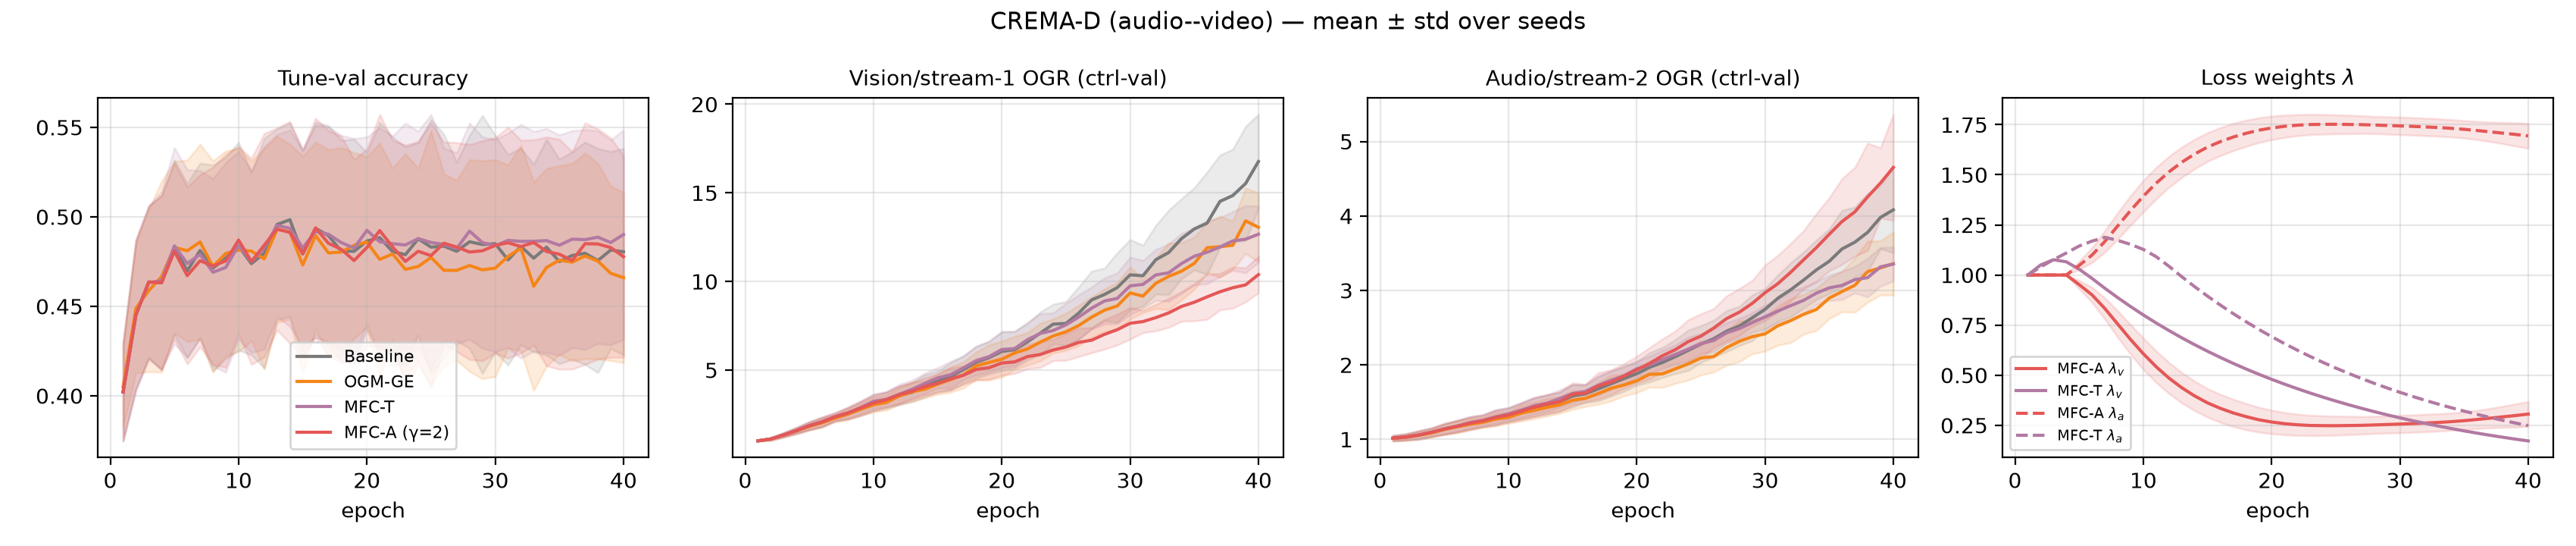
\includegraphics[width=\textwidth]{images/dynamics_crema_av.png}
\caption{\textbf{Intermediate evidence on CREMA-D audio--video} (mean $\pm$ std over 10 seeds). From left: tune-split accuracy; OGR of the video stream and of the audio stream on $\mathcal{D}_{\mathrm{cv}}$; loss weights of MFC-A (solid: $\lambda_v$, dashed: $\lambda_a$) and MFC-T.}
\label{fig:dyn_av}
\end{figure*}

\begin{figure*}[t]
\centering
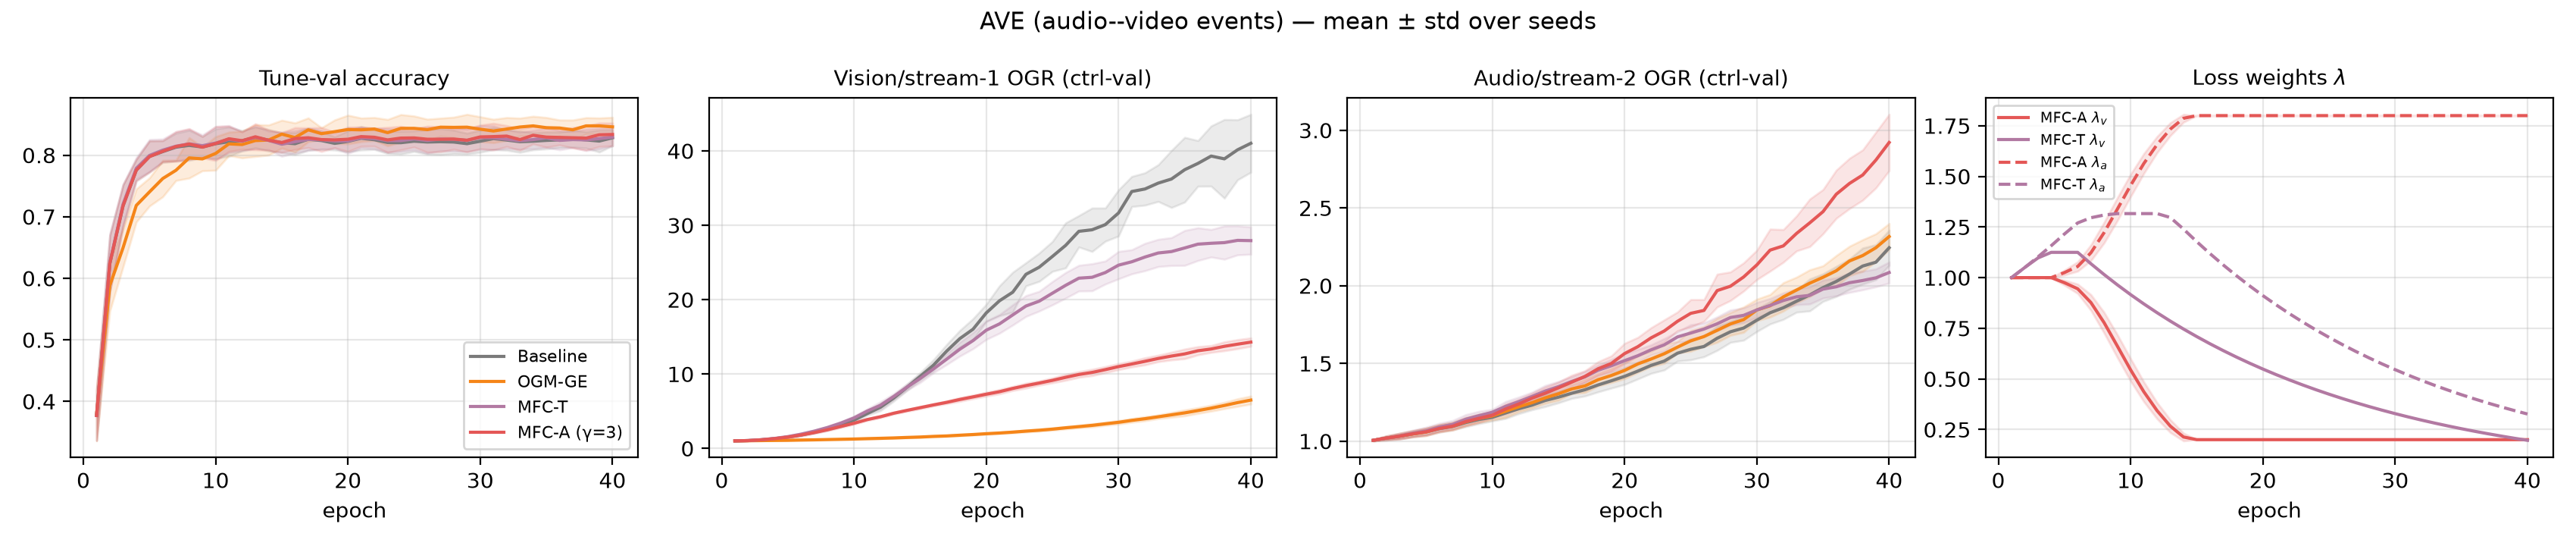
\includegraphics[width=\textwidth]{images/dynamics_ave.png}
\caption{\textbf{Intermediate evidence on AVE} (mean $\pm$ std over 10 seeds). Panels as in Fig.~\ref{fig:dyn_av}. The video OGR of the baseline grows to about 41; MFC-A ($\gamma{=}3$) moves the video weight to its lower bound within a few epochs after warm-up and keeps the video OGR at about 14.}
\label{fig:dyn_ave}
\end{figure*}

\begin{figure*}[t]
\centering
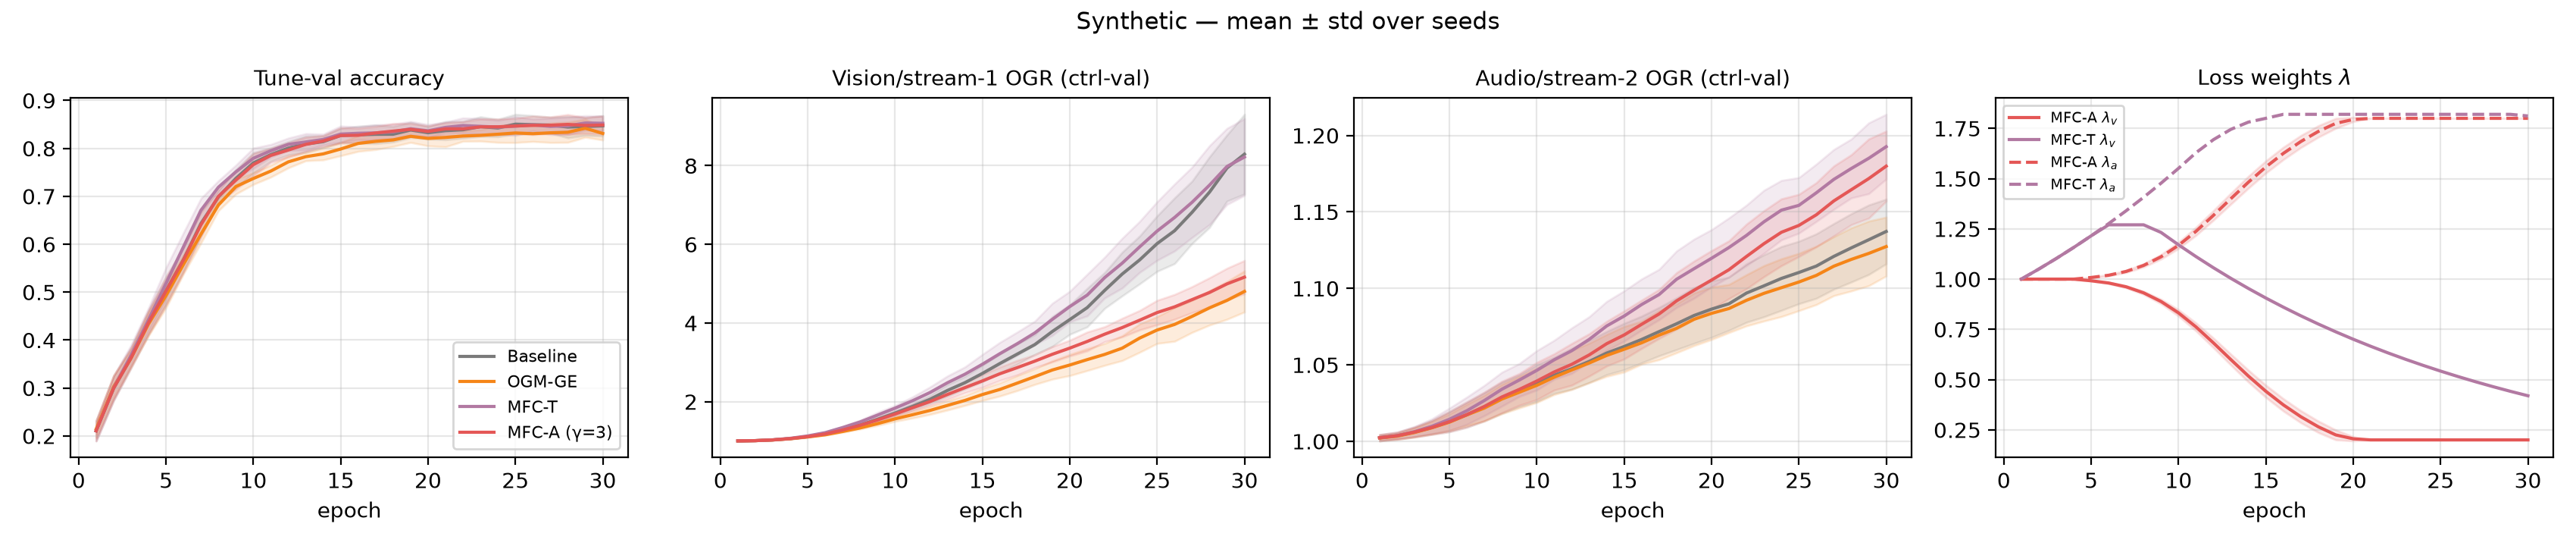
\includegraphics[width=\textwidth]{images/dynamics_synthetic.png}
\caption{\textbf{Intermediate evidence on the synthetic benchmark} (mean $\pm$ std over 10 seeds). Panels as in Fig.~\ref{fig:dyn_av}. The OGR of the easy stream grows several-fold while that of the hard stream stays near 1.2; MFC-A transfers auxiliary weight from the first stream to the second.}
\label{fig:dyn_syn}
\end{figure*}

\subsection*{Gradient-level evidence}
To test the mechanism directly, we logged at the end of every epoch, on a fixed probe of 512 training samples, the gradient norms that each encoder receives from the joint loss ($\|\nabla_{\theta_m}\mathcal{L}_{\mathrm{joint}}\|$) and from its own unimodal loss ($\|\nabla_{\theta_m}\mathcal{L}_m\|$). The probe uses inference mode and draws no random numbers, and rerunning all 160 main-comparison runs with this logging reproduced every previously reported result exactly. Figure~\ref{fig:grad} shows AVE.

In the AVE baseline, the audio encoder's share of the joint-loss gradient, $\|\nabla_{\theta_a}\mathcal{L}_{\mathrm{joint}}\|/(\|\nabla_{\theta_v}\mathcal{L}_{\mathrm{joint}}\|+\|\nabla_{\theta_a}\mathcal{L}_{\mathrm{joint}}\|)$, falls from 0.46 in the first epoch to about 0.23 from epoch 20 onwards: the audio encoder is partly, though not completely, starved by the joint loss. MFC-A acts where it was designed to act. After warm-up, the effective auxiliary gradient $\lambda_m\|\nabla_{\theta_m}\mathcal{L}_m\|$ reaching the video encoder is 54\% lower than in the baseline and that reaching the audio encoder is 66\% higher (both $p<10^{-7}$); on CREMA-D the corresponding changes are $-55\%$ and $+45\%$ ($p<10^{-8}$). The joint-loss gradient share, however, is almost unchanged on AVE (0.229 vs.\ 0.236), because MFC-A does not re-weight $\mathcal{L}_{\mathrm{joint}}$. OGM-GE, which scales the encoder gradients directly, is the only method that measurably raises the audio-to-video ratio of the joint-loss gradient norms (by 43\%, $p\approx10^{-7}$). This explains both why MFC-A reduces the OGR-measured imbalance and why its effect on accuracy and robustness is smaller than OGM-GE's on AVE, and it identifies re-weighting of the joint term as the main lever for a stronger version of the controller.

\begin{figure*}[t]
\centering
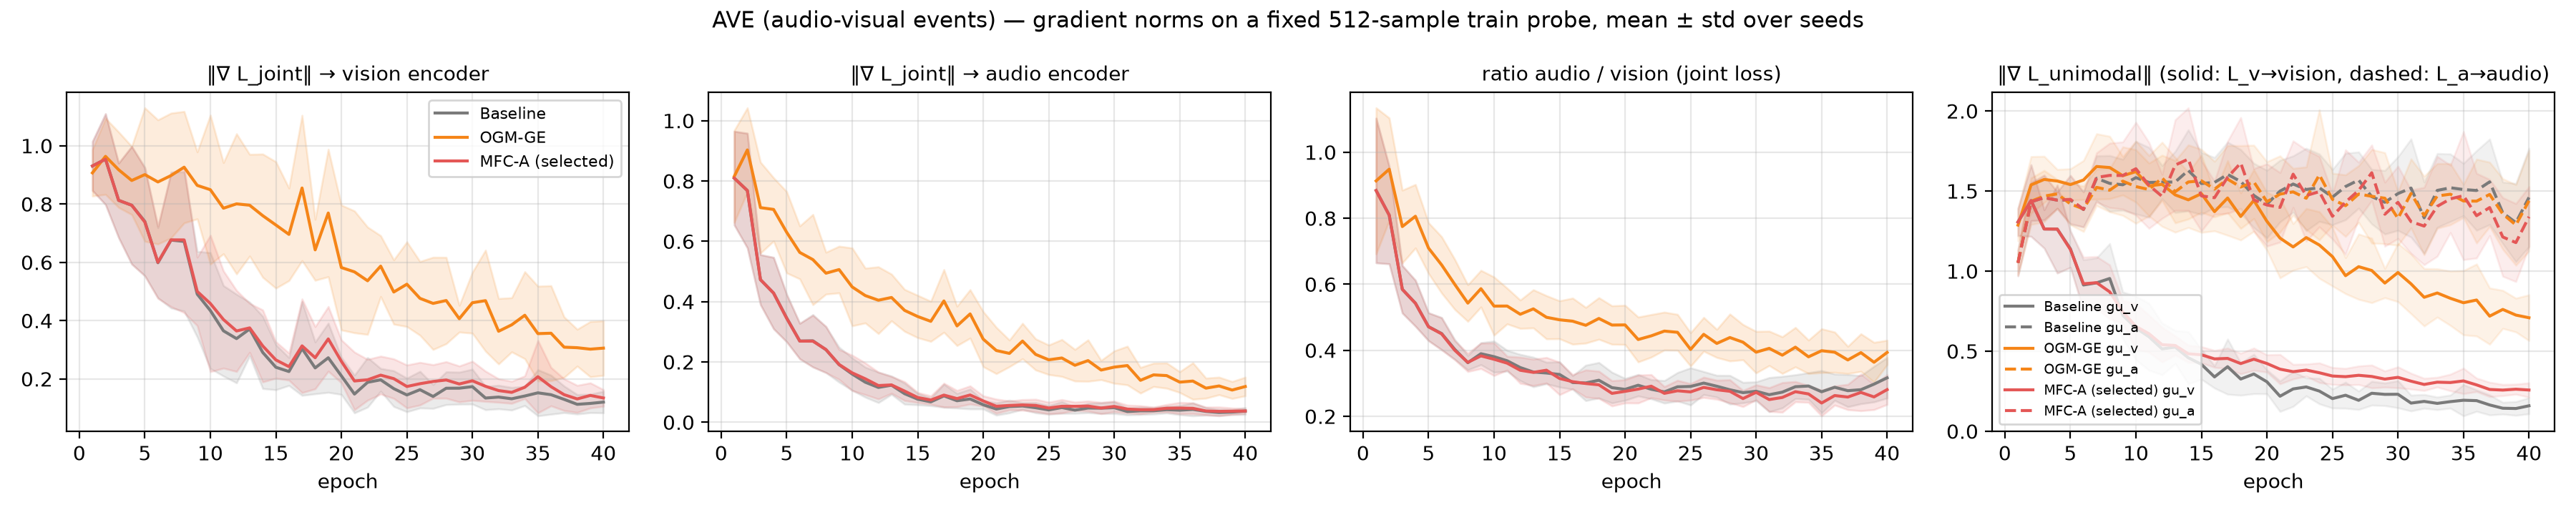
\includegraphics[width=\textwidth]{images/gradnorm_ave.png}
\caption{\textbf{Gradient norms on AVE} (fixed 512-sample training probe, mean $\pm$ std over 10 seeds). From left: joint-loss gradient reaching the video encoder and the audio encoder; their ratio (audio/video); unimodal-loss gradient of each encoder (solid: video, dashed: audio). The corresponding figure for CREMA-D is released with the code.}
\label{fig:grad}
\end{figure*}

\subsection*{Follow-up: stronger variants guided by the gradient evidence}
The gradient-level analysis identified why MFC-A's effect is limited: it re-weights only the auxiliary losses, while the joint loss, which dominates the encoders' gradients, is untouched. We therefore designed, after that analysis and before running them, two variants that act on the joint-loss gradient as well, and evaluated both under the unchanged protocol (ten paired seeds, settings chosen by the pre-registered rule on $\mathcal{D}_{\mathrm{cv}}$ and $\mathcal{D}_{\mathrm{tune}}$, untouched test set). \textbf{MFC-J} applies the MFC-A weights $\lambda_m$ also to the joint-loss gradient that enters the fusion layer from each encoder ($\gamma\in\{1,2,3\}$). \textbf{MFC-OG} keeps MFC-A and adds OGM-GE gradient modulation\cite{peng2022balanced}, but applies it only when the more confident modality is also the one with the higher smoothed OGR, that is, only when its confidence comes from memorisation ($\alpha\in\{0.3,0.8\}$, $\gamma\in\{1,3\}$). Because these variants were motivated by results we had already seen, we report them as a follow-up, and we report both of them on every dataset, including where they fail. All runs in this subsection, including the reference methods, were made on the same workstation; for the synthetic and spectrogram datasets the reference numbers are therefore reruns and differ slightly from Tables~\ref{tab:main_syn} and \ref{tab:main_spec}.

\begin{table*}[t]
\caption{\textbf{Follow-up variants} (test set, 10 seeds, means; all runs on one machine). MFC-J and MFC-OG use the setting chosen by the pre-registered rule; $^{\dagger}$: no setting passed the rule (tuning accuracy more than 0.5 points below the baseline), so the setting with the best tuning accuracy is shown. $^{*}$: paired $t$-test $p<0.05$ against the baseline. Bold: best mean per column.}
\label{tab:variants}
\centering
\footnotesize
\setlength{\tabcolsep}{2.5pt}
\begin{tabular}{@{}lcccccccccccc@{}}
\toprule
& \multicolumn{3}{c}{\textbf{AVE}} & \multicolumn{3}{c}{\textbf{CREMA-D audio--video}} & \multicolumn{3}{c}{\textbf{Synthetic}} & \multicolumn{3}{c}{\textbf{Spectrogram views}} \\
\cmidrule(lr){2-4}\cmidrule(lr){5-7}\cmidrule(lr){8-10}\cmidrule(lr){11-13}
\textbf{Method} & Acc & Gap & Rob@1 & Acc & Gap & Rob@1 & Acc & Gap & Rob@1 & Acc & Gap & Rob@1 \\ \midrule
Baseline & 79.9 & 25.87 & 74.9 & 49.7 & 3.73 & 43.4 & 84.1 & 6.03 & 48.9 & 49.1 & 1.21 & 35.9 \\
Gradient Blending & 81.0$^{*}$ & 5.33$^{*}$ & 76.6$^{*}$ & \textbf{52.1$^{*}$} & \textbf{1.17$^{*}$} & \textbf{47.3$^{*}$} & 84.0 & 4.23$^{*}$ & \textbf{49.9$^{*}$} & \textbf{50.7$^{*}$} & \textbf{0.51$^{*}$} & \textbf{39.8$^{*}$} \\
OGM-GE & 82.4$^{*}$ & 2.51$^{*}$ & 78.8$^{*}$ & 50.6 & 2.77 & 44.4 & 82.7$^{*}$ & 3.29$^{*}$ & 49.2 & 50.0 & 0.98 & 37.9$^{*}$ \\
MFC-A & 80.2 & 9.50$^{*}$ & 75.9$^{*}$ & 48.8 & 2.90 & 43.2 & 84.4 & 3.74$^{*}$ & 49.6 & 49.1 & 1.12 & 36.5 \\
MFC-J & 80.5 & 5.99$^{*}$ & 76.1$^{*}$ & 49.3$^{\dagger}$ & 4.15 & 43.5 & \textbf{84.5} & 3.13$^{*}$ & 49.7 & 49.8 & 0.99 & 36.2 \\
MFC-OG & \textbf{82.5$^{*}$} & \textbf{1.42$^{*}$} & \textbf{79.7$^{*}$} & 50.0 & 1.71 & 44.2 & 82.2$^{*}$$^{\dagger}$ & \textbf{2.20$^{*}$} & 49.2 & 49.6 & 0.72 & 37.9$^{*}$ \\
\bottomrule
\end{tabular}
\end{table*}

Table~\ref{tab:variants} shows that acting on the joint-loss gradient helps where the analysis predicted. On AVE, MFC-OG improves on the baseline on every metric (accuracy $+2.7$, OGR gap $-24.4$, robustness $+4.8$, blur $+12.5$, low light $+11.0$, missing video $+9.3$ points; all $p<0.01$) and matches OGM-GE, the strongest method on this dataset: accuracy and robustness to blur, low light and missing video are statistically indistinguishable, the OGR gap is lower (1.42 vs.\ 2.51, $p{=}0.08$), and robustness to feature noise is higher (79.7 vs.\ 78.8\%, $p{=}0.04$). It is also more accurate and more robust than Gradient Blending on AVE (all $p<0.01$). On the synthetic benchmark, MFC-J is the most accurate method (84.5\%; $+1.9$ over OGM-GE, $p{=}0.001$) with a lower OGR gap than Gradient Blending ($p{=}0.01$). The variants do not fix everything. On CREMA-D neither improves significantly on the baseline and Gradient Blending remains clearly best; no MFC-J setting passes the selection rule on CREMA-D, and no MFC-OG setting passes it on the synthetic benchmark, where its best setting loses 1.9 accuracy points, as OGM-GE does. Neither variant is therefore uniformly better than MFC-A. We read these results as evidence that the OGR signal is useful for deciding \emph{when} to slow a dominant modality: gating OGM-GE by OGR retained all of its benefit on AVE while reducing the imbalance further. Finally, because Gradient Blending's advantage on CREMA-D comes from allocations that MFC-A's lower bound of 0.2 cannot reach, we also re-ran all three controllers with the bounds widened to $[0,2]$ and $\gamma\in\{1,3,5\}$ (480 further runs, same rule, all on one machine). With the zero lower bound, MFC-A ($\gamma{=}5$, chosen by the rule on every dataset) is never significantly worse than the baseline on any measured quantity (accuracy, unimodal accuracies, OGR gap, feature noise, blur, occlusion, low light, JPEG compression and missing video) on any of the four datasets, and it is significantly better on at least one of them on each dataset: the OGR gap falls by 84\% on AVE ($p{=}0.01$) and by 58\% on the synthetic benchmark ($p<0.001$), and robustness improves on both CREMA-D settings ($p<0.03$). It remains behind Gradient Blending on CREMA-D (accuracy $-1.9$ points, $p{=}0.04$; robustness $-3.0$, $p{=}0.002$), so widening the bounds narrows but does not close that gap.

\subsection*{Component ablation}
Table~\ref{tab:ablation} isolates each component of MFC-A. ``Static weights'' fixes $\lambda$ at MFC-A's average trajectory value for the whole run, which tests whether the \emph{dynamics} matter or only the final allocation. ``Raw gap signal'' replaces $\widetilde{\OGR}_m$ in Eq.~(\ref{eq:target}) by $1+\max(\tilde G_m,0)$, which keeps everything else unchanged and removes only the scale normalisation. ``Throttle only'' and ``Amplify only'' restrict the target to $\pi_m\le1$ and $\pi_m\ge1$, respectively.

\begin{table*}[t]
\caption{\textbf{Component ablation} (test set, 10 seeds, mean\pmm std), plain law $\gamma{=}1$. $^{*}$: paired $t$-test $p<0.05$ against full MFC-A ($\gamma{=}1$).}
\label{tab:ablation}
\centering
\footnotesize
\setlength{\tabcolsep}{3pt}
\begin{tabular}{@{}lccc@{\hskip 8pt}ccc@{\hskip 8pt}ccc@{}}
\toprule
& \multicolumn{3}{c}{\textbf{CREMA-D audio--video}} & \multicolumn{3}{c}{\textbf{AVE}} & \multicolumn{3}{c}{\textbf{Synthetic}} \\
\cmidrule(lr){2-4}\cmidrule(lr){5-7}\cmidrule(lr){8-10}
\textbf{Variant} & \textbf{Acc} & \textbf{OGR gap}$\downarrow$ & \textbf{Rob@1.0} & \textbf{Acc} & \textbf{OGR gap}$\downarrow$ & \textbf{Rob@1.0} & \textbf{Acc} & \textbf{OGR gap}$\downarrow$ & \textbf{Rob@1.0} \\ \midrule
Baseline (no control) & 49.7$\pm$5.8 & 3.73$\pm$3.60 & 43.4$\pm$3.3 & 79.9$\pm$1.8 & 25.87$\pm$22.28 & 74.9$\pm$1.2 & 84.1$\pm$1.1 & 6.01$\pm$1.36 & 48.8$\pm$2.1 \\
Static weights ($\bar\lambda$ of MFC-A) & 49.6$\pm$5.1 & 2.36$\pm$1.78 & 44.6$\pm$3.2 & 81.0$\pm$1.3 & 7.89$\pm$6.91 & 76.4$\pm$1.6 & 84.0$\pm$1.4 & 4.62$\pm$1.18 & 49.8$\pm$2.9 \\
Raw gap signal instead of OGR & 48.9$\pm$5.7 & 3.63$\pm$2.70 & 43.1$\pm$3.9 & 79.5$\pm$1.7 & 23.51$\pm$19.32 & 73.8$\pm$1.4 & 84.4$\pm$1.6 & 5.96$\pm$1.16 & 48.7$\pm$2.2 \\
Throttle rule only ($\lambda\le1$) & 49.7$\pm$6.0 & 3.36$\pm$2.12 & 43.4$\pm$3.0 & 80.2$\pm$1.2 & 12.66$\pm$8.66 & 75.2$\pm$1.1 & 84.1$\pm$1.4 & 5.06$\pm$1.11 & 49.8$\pm$2.3 \\
Amplify rule only ($\lambda\ge1$) & 49.2$\pm$5.4 & 4.30$\pm$3.49 & 43.3$\pm$3.6 & 79.4$\pm$1.7 & 26.18$\pm$21.67 & 74.0$\pm$1.4 & 84.0$\pm$1.9 & 5.69$\pm$1.37 & 49.0$\pm$2.2 \\
No warm-up & 48.9$\pm$5.7 & 3.28$\pm$2.35 & 43.4$\pm$3.3 & 79.9$\pm$1.5 & 14.11$\pm$9.07 & 74.7$\pm$1.3 & 84.6$\pm$1.3 & 4.71$\pm$1.06 & 49.9$\pm$2.3 \\
No EMA & 50.1$\pm$6.1 & 2.56$\pm$1.55 & 43.9$\pm$3.2 & 80.1$\pm$1.1 & 12.10$\pm$7.90 & 75.0$\pm$1.4 & 84.4$\pm$1.5 & 4.81$\pm$1.05 & 49.5$\pm$2.2 \\
No window ($W{=}1$) & 49.6$\pm$5.5 & 3.75$\pm$2.80 & 43.6$\pm$3.3 & 80.3$\pm$1.4 & 10.54$\pm$5.89 & 74.8$\pm$1.2 & 84.6$\pm$1.4 & 4.87$\pm$1.21 & 49.5$\pm$2.1 \\
Running train loss (no extra pass) & 49.3$\pm$5.5 & 3.13$\pm$2.26 & 43.7$\pm$3.0 & 79.9$\pm$2.0 & 17.75$\pm$11.37 & 74.4$\pm$1.6 & 84.0$\pm$1.3 & 5.70$\pm$1.54 & 49.4$\pm$2.8 \\
\textbf{MFC-A (full)} & 49.3$\pm$5.4 & 2.98$\pm$2.38 & 43.8$\pm$3.3 & 80.2$\pm$1.6 & 14.47$\pm$8.48 & 74.8$\pm$1.8 & 84.5$\pm$1.7 & 5.11$\pm$1.12 & 49.3$\pm$2.0 \\
\bottomrule
\end{tabular}
\end{table*}

The ablation uses the plain law ($\gamma{=}1$) so that each component is isolated. Four observations stand out. (i) \emph{OGR vs.\ raw gap.} Replacing OGR with the raw gap weakens balancing on all three datasets with unequal loss scales (AVE 23.5 vs.\ 14.5, $p{=}0.05$; CREMA-D 3.63 vs.\ 2.98; synthetic 5.96 vs.\ 5.11) and significantly lowers the hard stream's head accuracy on the synthetic data ($p{=}0.025$). On the spectrogram control, where the two views have similar loss scales, the two signals behave alike (1.23 vs.\ 1.32). This is what Proposition~\ref{prop:scale} predicts: normalisation matters when the loss scales of the modalities differ. (ii) \emph{Throttle vs.\ amplify.} Throttling alone retains essentially the full effect (AVE gap 12.7, synthetic 5.06), whereas amplifying alone is weaker and on AVE and CREMA-D does not reduce the gap at all (26.2 and 4.30, versus 25.9 and 3.73 for the baseline). The active ingredient is therefore the reduction of the overfitting modality's auxiliary weight. (iii) \emph{Dynamic vs.\ static.} Fixing $\lambda$ at MFC-A's average allocation from the start gives similar or better balance (AVE 7.9, CREMA-D 2.36, synthetic 4.62) and on AVE slightly better robustness ($p{=}0.007$), with the same accuracy. The value of the closed loop is that it \emph{finds} this allocation within a single run, whereas a static schedule has to be known in advance or estimated from extra runs, as in Gradient Blending. (iv) \emph{Smoothing.} Removing warm-up, EMA or the window changes no metric significantly, and the running-loss variant performs comparably on audio--video at a fraction of the monitoring cost.

\subsection*{Sensitivity to hyper-parameters}
Table~\ref{tab:sens} varies one hyper-parameter at a time around the default ($W{=}5$, $\beta{=}0.7$, $T_w{=}3$, $[0.2,1.8]$) on all four datasets, reporting the tune-split accuracy that would be used for selection together with test accuracy and OGR gap. For the smoothing and timing hyper-parameters ($W$, $\beta$, $T_w$, clipping), test accuracy stays within 0.6 points of the default on every dataset, and no change is significant. The OGR gap varies more (for example, a longer warm-up lowers it on audio--video, 2.05 vs.\ 2.98, $p{=}0.17$), but without a consistent pattern across datasets. The control strength $\gamma$ has the largest effect: on the synthetic benchmark the gap falls monotonically from 5.11 ($\gamma{=}1$) to 3.56 ($\gamma{=}3$) at constant accuracy. Under the plain law, $\lambda$ never leaves $[0.2,1.8]$, so the clipping range acts only as a safety bound (practically identical results for $[0.1,5.0]$); with $\gamma\ge2$ the lower bound becomes active on the synthetic and audio--video data. The smoothing defaults were not fine-tuned, and the same values are used on every dataset.

\begin{table*}[t]
\caption{\textbf{Sensitivity of MFC-A} (10 seeds, means; standard deviations are in the released logs). Tune: accuracy on $\mathcal{D}_{\mathrm{tune}}$ (used for selection). Test: accuracy on $\mathcal{D}_{\mathrm{te}}$. Gap: test OGR gap.}
\label{tab:sens}
\centering
\footnotesize
\setlength{\tabcolsep}{2.5pt}
\begin{tabular}{@{}lcccccccccccc@{}}
\toprule
& \multicolumn{3}{c}{\textbf{CREMA-D audio--video}} & \multicolumn{3}{c}{\textbf{AVE}} & \multicolumn{3}{c}{\textbf{Synthetic}} & \multicolumn{3}{c}{\textbf{Spectrogram views}} \\
\cmidrule(lr){2-4}\cmidrule(lr){5-7}\cmidrule(lr){8-10}\cmidrule(lr){11-13}
\textbf{Setting} & Tune & Test & Gap & Tune & Test & Gap & Tune & Test & Gap & Tune & Test & Gap \\ \midrule
$\gamma$=1 (default law) & 51.4 & 49.3 & 2.98 & 84.2 & 80.2 & 14.47 & 85.8 & 84.5 & 5.11 & 52.3 & 49.3 & 1.32 \\
$\gamma$=2 & 51.8 & 48.8 & 2.90 & 84.4 & 80.4 & 11.16 & 85.9 & 84.5 & 4.25 & 52.3 & 49.3 & 1.25 \\
$\gamma$=3 & 51.2 & 50.1 & 2.16 & 84.2 & 80.2 & 9.50 & 85.8 & 84.3 & 3.56 & 52.3 & 49.1 & 1.34 \\
$W$=3 & 51.6 & 49.9 & 2.85 & 84.2 & 80.3 & 12.12 & 85.9 & 84.3 & 5.23 & 52.3 & 49.5 & 1.65 \\
$W$=5 (default) & 51.4 & 49.3 & 2.98 & 84.2 & 80.2 & 14.47 & 85.8 & 84.5 & 5.11 & 52.3 & 49.3 & 1.32 \\
$W$=10 & 51.4 & 49.5 & 3.38 & 84.3 & 80.0 & 17.73 & 85.7 & 84.4 & 5.39 & 52.4 & 49.3 & 1.28 \\
EMA 0.5 & 51.6 & 49.5 & 3.48 & 84.2 & 80.3 & 11.99 & 86.0 & 84.8 & 5.05 & 52.4 & 48.9 & 1.42 \\
EMA 0.7 (default) & 51.4 & 49.3 & 2.98 & 84.2 & 80.2 & 14.47 & 85.8 & 84.5 & 5.11 & 52.3 & 49.3 & 1.32 \\
EMA 0.9 & 52.0 & 49.5 & 3.31 & 84.0 & 79.9 & 19.58 & 85.8 & 84.7 & 6.00 & 52.4 & 49.1 & 1.27 \\
Warm-up 0 & 51.6 & 48.9 & 3.28 & 84.2 & 79.9 & 14.11 & 86.1 & 84.6 & 4.71 & 52.2 & 49.2 & 1.41 \\
Warm-up 3 (default) & 51.4 & 49.3 & 2.98 & 84.2 & 80.2 & 14.47 & 85.8 & 84.5 & 5.11 & 52.3 & 49.3 & 1.32 \\
Warm-up 5 & 51.3 & 49.8 & 2.05 & 84.3 & 80.2 & 15.09 & 85.7 & 84.0 & 4.57 & 52.2 & 49.3 & 1.23 \\
Clip [0.5,1.5] & 51.5 & 49.4 & 2.96 & 84.1 & 80.1 & 15.29 & 85.6 & 84.2 & 5.20 & 52.3 & 49.3 & 1.32 \\
Clip [0.2,1.8] (default) & 51.4 & 49.3 & 2.98 & 84.2 & 80.2 & 14.47 & 85.8 & 84.5 & 5.11 & 52.3 & 49.3 & 1.32 \\
Clip [0.1,5.0] & 51.4 & 49.3 & 2.98 & 84.1 & 80.2 & 14.47 & 85.8 & 84.5 & 5.11 & 52.3 & 49.3 & 1.32 \\
\bottomrule
\end{tabular}
\end{table*}

\subsection*{Effect of encoder capacity}
Table~\ref{tab:capacity} widens the first-stream encoder of the synthetic model from 128 to 1024 hidden units (plain law, $\gamma{=}1$). A wider dominant encoder memorises faster: the baseline's OGR gap grows from 6.0 to 93.6. MFC-A's relative advantage grows accordingly: it reduces the gap by 15\% at 128 units, by 35\% at 256 ($p{=}0.015$), by 52\% at 512 ($p{=}0.002$) and by 55\% at 1024 units (93.6 to 41.7, $p{=}0.008$), and robustness at $\sigma{=}1$ improves significantly for widths of 256 and above (+0.6 to +1.1 points). Accuracy differences remain within $\pm0.8$ points and are not significant at any width. The first submission reported a +3.1-point accuracy gain at 1024 units from a single run; with ten seeds this gain is +0.76 points ($p{=}0.09$), and we withdraw the earlier claim.

\begin{table}[t]
\caption{\textbf{Capacity study} (synthetic, 10 seeds). Width of the first-stream hidden layer. $\Delta$: MFC-A minus baseline (paired $p$-value in parentheses).}
\label{tab:capacity}
\centering
\footnotesize
\setlength{\tabcolsep}{2.5pt}
\begin{tabular}{@{}lcccccc@{}}
\toprule
\textbf{Width} & \textbf{Base Acc} & \textbf{MFC-A Acc} & \textbf{$\Delta$Acc ($p$)} & \textbf{Base gap} & \textbf{MFC-A gap} & \textbf{$\Delta$Rob@1 ($p$)} \\ \midrule
128 & 84.1$\pm$1.1 & 84.5$\pm$1.7 & +0.32 (0.35) & 6.01$\pm$1.36 & 5.11$\pm$1.12 & +0.48 (0.18) \\
256 & 84.9$\pm$1.1 & 85.5$\pm$0.8 & +0.62 (0.07) & 19.93$\pm$7.75 & 12.94$\pm$3.95 & +1.06 (0.02) \\
512 & 84.8$\pm$0.9 & 85.2$\pm$1.2 & +0.36 (0.17) & 60.98$\pm$24.41 & 29.09$\pm$5.53 & +0.56 (0.02) \\
1024 & 82.9$\pm$1.8 & 83.6$\pm$1.5 & +0.76 (0.09) & 93.56$\pm$57.97 & 41.66$\pm$13.88 & +0.66 (0.05) \\
\bottomrule
\end{tabular}
\end{table}

\subsection*{Robustness to visual degradation}
Figure~\ref{fig:rob} shows accuracy as the first stream is increasingly corrupted. On the synthetic benchmark, MFC-A ($\gamma{=}3$) is the most robust method at $\sigma{=}1$ (49.7\%, $+0.9$ over the baseline, $p{=}0.04$), although differences between methods are within about one point. On AVE, MFC-A improves robustness to feature noise, blur and low light significantly over the baseline, but OGM-GE improves it much more. On audio--video CREMA-D only Gradient Blending improves robustness to feature noise ($+3.9$ points at $\sigma{=}1$). On CREMA-D the pixel-level degradations are more damaging than removing the video altogether: blur and occlusion reduce every method to 23--28\%, whereas replacing the video features by their mean (``No video'') leaves 44\%. On vision-dominant AVE the opposite holds: removing the video is the most damaging condition (27--36\%), because the audio stream alone is weak. Corrupted frames produce out-of-distribution features that actively mislead the fusion head, and no loss-weighting method, MFC-A included, protects against this. Handling such inputs requires detecting or gating the corrupted modality, or training with adverse-condition data\cite{lan2025sustechgan}, which is complementary to balancing. Table~\ref{tab:severity} grades the three pixel-level degradations on AVE at three severities. MFC-A is 1--2 points above the baseline at every severity (significant for blur s3 and low light s1--s2) but below OGM-GE everywhere, with the gap widening with severity (blur s3: $-9.7$ points, $p<10^{-4}$), and Gradient Blending is also better at most severities. On CREMA-D (tables released with the code) no method differs significantly from MFC-A at the highest severity. JPEG compression (Table~\ref{tab:jpeg}) shows the same pattern: MFC-A is not significantly more robust than the baseline at any quality level except a $+0.9$-point gain at quality 30 on AVE ($p{=}0.049$), whereas OGM-GE gains $+3.7$, $+5.4$ and $+11.6$ points over the baseline on AVE at qualities 30, 15 and 5 (all $p<0.001$) and Gradient Blending is the most robust method on CREMA-D at qualities 30 and 15. We therefore do not claim a robustness advantage for MFC-A over the strongest baselines. At $\sigma\ge2$ all methods converge towards the accuracy that the second stream supports on its own, as expected when the first stream carries almost no information.

\begin{table*}[t]
\caption{\textbf{Robustness to graded pixel-level degradations on AVE} (test accuracy, 10 seeds, mean\pmm std). Severities s1/s2/s3: blur $\sigma$ = 2/4/6 (kernel 21); occluder 56/84/112 px; low light = brightness $\times$0.5/0.35/0.25 with noise std 0.02/0.035/0.05. $^{*}$: paired $t$-test $p<0.05$ against the selected MFC-A. Bold: best mean.}
\label{tab:severity}
\centering
\footnotesize
\setlength{\tabcolsep}{3pt}
\begin{tabular}{@{}lccccccccc@{}}
\toprule
& \multicolumn{3}{c}{\textbf{Blur}} & \multicolumn{3}{c}{\textbf{Occlusion}} & \multicolumn{3}{c}{\textbf{Low light}} \\
\cmidrule(lr){2-4}\cmidrule(lr){5-7}\cmidrule(lr){8-10}
\textbf{Method} & s1 & s2 & s3 & s1 & s2 & s3 & s1 & s2 & s3 \\ \midrule
Baseline & 71.2$\pm$1.8 & 53.1$\pm$3.0 & 39.4$\pm$4.8$^{*}$ & 76.4$\pm$1.9 & 72.8$\pm$1.9 & 65.6$\pm$1.7 & 74.5$\pm$1.2$^{*}$ & 65.4$\pm$2.1$^{*}$ & 50.9$\pm$2.1 \\
Gradient Blending & 74.0$\pm$2.3 & 56.7$\pm$4.3$^{*}$ & 43.5$\pm$6.6 & 77.7$\pm$1.5 & 75.3$\pm$1.2$^{*}$ & 68.2$\pm$2.5$^{*}$ & 76.8$\pm$1.5$^{*}$ & 68.8$\pm$1.7$^{*}$ & 57.0$\pm$3.0$^{*}$ \\
Uncertainty weighting & 68.1$\pm$1.6$^{*}$ & 46.6$\pm$4.0$^{*}$ & 32.3$\pm$4.5$^{*}$ & 73.8$\pm$1.2$^{*}$ & 70.2$\pm$1.6$^{*}$ & 62.2$\pm$2.8$^{*}$ & 72.6$\pm$1.9$^{*}$ & 62.8$\pm$2.3$^{*}$ & 49.2$\pm$2.2$^{*}$ \\
MMPareto & 70.7$\pm$1.8$^{*}$ & 50.8$\pm$3.7$^{*}$ & 37.7$\pm$5.4$^{*}$ & 75.6$\pm$1.6$^{*}$ & 72.3$\pm$1.5 & 64.7$\pm$1.9$^{*}$ & 74.7$\pm$1.2$^{*}$ & 65.6$\pm$2.4$^{*}$ & 51.1$\pm$2.8 \\
OGM-GE ($\alpha$=0.8) & \textbf{76.2$\pm$0.7$^{*}$} & \textbf{61.8$\pm$3.0$^{*}$} & \textbf{51.2$\pm$4.9$^{*}$} & \textbf{79.4$\pm$1.3$^{*}$} & \textbf{77.1$\pm$1.0$^{*}$} & \textbf{71.6$\pm$1.9$^{*}$} & \textbf{78.5$\pm$1.2$^{*}$} & \textbf{71.9$\pm$1.6$^{*}$} & \textbf{61.3$\pm$2.2$^{*}$} \\
MFC-T (threshold) & 72.0$\pm$1.9 & 53.3$\pm$2.7 & 39.8$\pm$4.1 & 76.5$\pm$0.8 & 73.4$\pm$1.0 & 65.9$\pm$1.5 & 75.1$\pm$1.3 & 66.3$\pm$1.4$^{*}$ & 51.4$\pm$2.2 \\
MFC-A ($\gamma$=1) & 72.1$\pm$1.6 & 52.9$\pm$2.6 & 40.2$\pm$4.7 & 76.5$\pm$1.0 & 73.6$\pm$1.5 & 66.0$\pm$1.4 & 75.1$\pm$1.3 & 66.4$\pm$2.0$^{*}$ & 51.3$\pm$2.8 \\
\textbf{MFC-A} ($\gamma$=3, selected) & 72.5$\pm$1.2 & 54.1$\pm$2.4 & 41.5$\pm$5.0 & 77.1$\pm$1.3 & 73.4$\pm$1.7 & 66.4$\pm$1.4 & 75.4$\pm$1.2 & 67.2$\pm$1.6 & 52.1$\pm$1.8 \\
\bottomrule
\end{tabular}
\end{table*}

\begin{table*}[t]
\caption{\textbf{Robustness to JPEG compression of the video frames} (test accuracy, 10 seeds, mean\pmm std). Each frame is JPEG-encoded and decoded (Pillow, libjpeg, 4:2:0 chroma subsampling) before encoding by ResNet-18. OGM-GE uses the $\alpha$ selected per dataset (0.3 on CREMA-D, 0.8 on AVE). $^{*}$: paired $t$-test $p<0.05$ against the selected MFC-A. Bold: best mean per column.}
\label{tab:jpeg}
\centering
\footnotesize
\begin{tabular}{@{}lcccccc@{}}
\toprule
& \multicolumn{3}{c}{\textbf{CREMA-D audio--video}} & \multicolumn{3}{c}{\textbf{AVE}} \\
\cmidrule(lr){2-4}\cmidrule(lr){5-7}
\textbf{Method} & $q{=}30$ & $q{=}15$ & $q{=}5$ & $q{=}30$ & $q{=}15$ & $q{=}5$ \\ \midrule
Baseline & 36.3$\pm$2.9 & 34.4$\pm$3.5 & \textbf{23.6$\pm$4.4} & 76.4$\pm$2.0$^{*}$ & 70.9$\pm$1.2 & 40.3$\pm$2.6 \\
Gradient Blending & \textbf{39.6$\pm$2.6$^{*}$} & \textbf{37.2$\pm$4.0$^{*}$} & 21.9$\pm$2.8 & 78.2$\pm$1.6$^{*}$ & 73.9$\pm$1.6$^{*}$ & 45.1$\pm$3.0$^{*}$ \\
Uncertainty weighting & 35.1$\pm$3.2 & 33.5$\pm$3.8 & 22.3$\pm$4.9 & 75.6$\pm$1.8 & 69.3$\pm$2.6 & 39.4$\pm$3.5 \\
MMPareto & 35.3$\pm$3.4 & 33.1$\pm$5.2 & 21.6$\pm$2.7 & 76.2$\pm$1.7 & 70.6$\pm$1.1$^{*}$ & 40.6$\pm$2.4 \\
OGM-GE & 34.6$\pm$3.0 & 31.9$\pm$4.3 & 22.8$\pm$5.7 & \textbf{80.1$\pm$1.2$^{*}$} & \textbf{76.3$\pm$0.9$^{*}$} & \textbf{51.9$\pm$2.6$^{*}$} \\
MFC-T (threshold) & 34.9$\pm$3.3 & 33.5$\pm$3.5 & 23.0$\pm$4.0 & 76.8$\pm$1.4 & 70.8$\pm$1.7 & 41.3$\pm$1.4 \\
MFC-A ($\gamma$=1) & 35.4$\pm$3.2 & 33.7$\pm$4.1 & 22.7$\pm$4.3 & 77.0$\pm$1.7 & 70.6$\pm$1.8$^{*}$ & 40.5$\pm$2.1 \\
\textbf{MFC-A} ($\gamma$=2, selected) & 35.2$\pm$3.4 & 33.8$\pm$3.3 & 22.1$\pm$3.1 & 77.3$\pm$1.7 & 71.3$\pm$1.6 & 41.1$\pm$1.8 \\
\bottomrule
\end{tabular}
\end{table*}

\begin{figure*}[t]
\centering
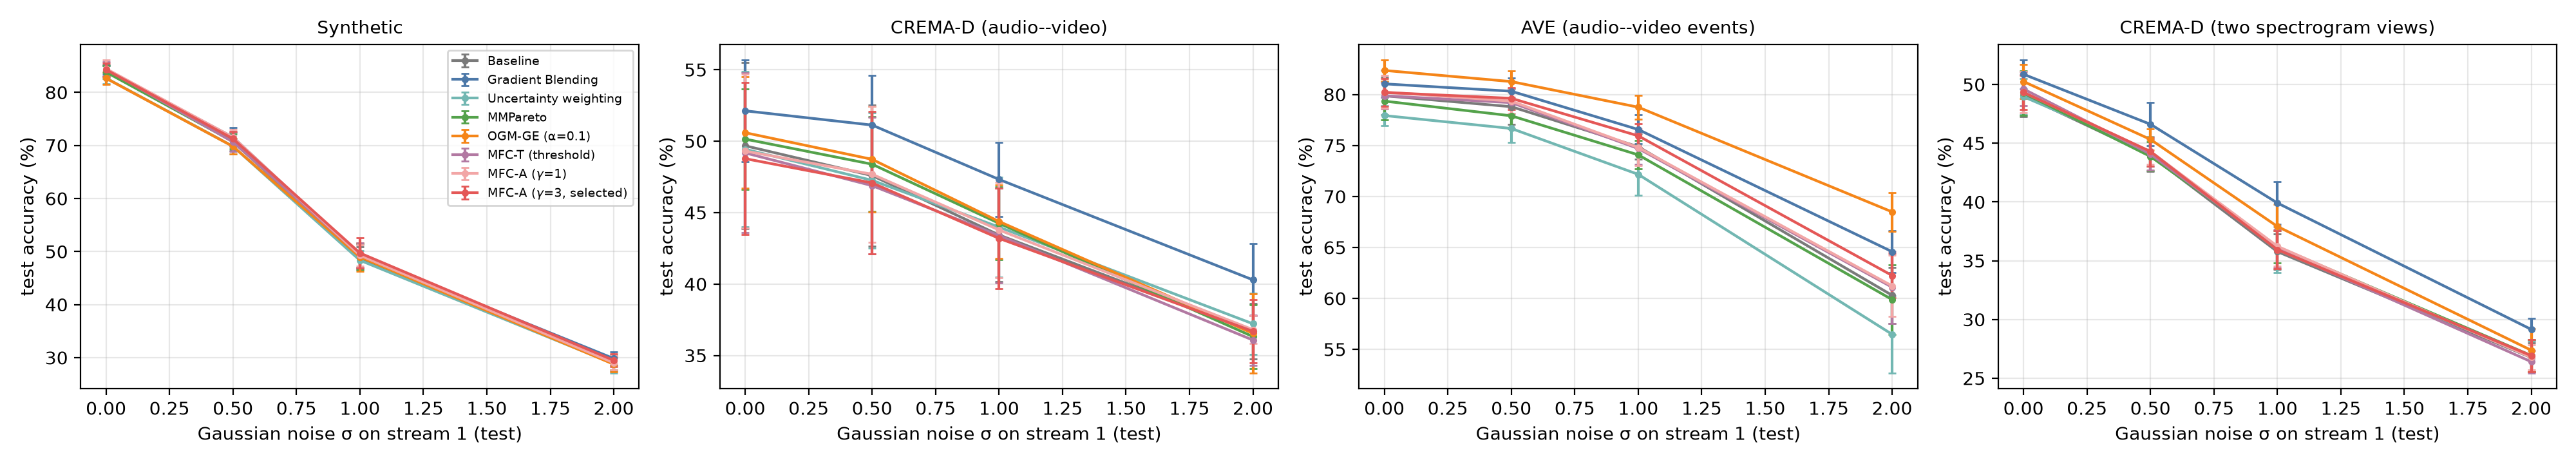
\includegraphics[width=\textwidth]{images/robustness.png}
\caption{\textbf{Robustness to Gaussian noise on the first stream} (test set, mean $\pm$ std over 10 seeds). Panels: synthetic, CREMA-D audio--video, AVE and spectrogram-view control (noise on the first-stream features).}
\label{fig:rob}
\end{figure*}

\subsection*{Computational cost}
Table~\ref{tab:cost} breaks the cost of each method into controller arithmetic, monitoring passes and method-specific work (probe training for Gradient Blending, per-batch gradient processing for OGM-GE and MMPareto). Times are single-thread CPU measurements averaged over ten runs (synthetic runs on a laptop CPU, CREMA-D runs on a 24-core workstation, so times are comparable within, not across, datasets); FLOPs are computed analytically from the layer sizes. We also measured memory (median of five fresh single-thread runs per method and dataset, with the allocator threshold fixed; per-method figures are released with the code). MFC-A's extra state is 1.27\,KB (its history buffer and weights), 0.06\% of the 2.18\,MB occupied by parameters, gradients and momentum buffers of the CREMA-D model; its traced Python heap grows by at most 0.005\,MB, and its peak resident memory lies within the run-to-run spread of the baseline on all four datasets. Of all methods, only MMPareto shows a measurable increase (1.7--2.7\,MB, from its transient per-step gradient copies). These measurements cover the fusion networks on frozen features, not the visual backbone. The controller arithmetic of MFC-A is negligible (a few milliseconds and 960 scalar operations per run). The monitoring passes are not negligible in FLOPs, at about 39\% of baseline training FLOPs on both models, because they run inference over the full training split every epoch. In wall-clock time, however, they add only 6.1\% (synthetic) and 18.4\% (audio--video) to the training time, since inference passes are batched and need no backward pass. The running variant removes the training pass and costs 1.8\% and 3.6\% extra time and 7.9\% and 7.5\% extra FLOPs, respectively; its balance is comparable on audio--video but weaker on the synthetic data (Table~\ref{tab:ablation}). Among the baselines, Gradient Blending's probe adds 24--132\% time, MMPareto's per-encoder gradient processing adds 103--168\%, and OGM-GE adds 45--67\% time but only about 1\% FLOPs, because its per-tensor gradient scaling and noise generation are dominated by per-operation overhead rather than arithmetic.

\begin{table*}[t]
\caption{\textbf{Cost per training run} (mean over 10 seeds). Ctrl: controller arithmetic time; Monitor: inference passes consumed by the controller; Method: method-specific work; Extra time: (Ctrl+Monitor+Method)/baseline training time; Ctrl ops: scalar operations; Extra FLOPs: (monitor+method FLOPs)/baseline training FLOPs.}
\label{tab:cost}
\centering
\footnotesize
\begin{tabular}{@{}llrrrrrr@{}}
\toprule
\textbf{Data} & \textbf{Method} & \textbf{Ctrl (ms)} & \textbf{Monitor (s)} & \textbf{Method (s)} & \textbf{Extra time (\%)} & \textbf{Ctrl ops} & \textbf{Extra FLOPs (\%)} \\ \midrule
Synthetic & Baseline & 0.0 & 0.00 & 0.00 & 0.0 & 0 & 0.0 \\
Synthetic & Gradient Blending & 0.0 & 0.00 & 1.78 & 131.5 & 0 & 21.6 \\
Synthetic & Uncertainty weighting & 0.0 & 0.00 & 0.00 & 0.0 & 0 & 0.0 \\
Synthetic & MMPareto & 0.3 & 0.00 & 1.40 & 103.0 & 0 & 63.2 \\
Synthetic & OGM-GE & 0.0 & 0.00 & 0.91 & 66.7 & 0 & 1.2 \\
Synthetic & MFC-T & 3.1 & 0.08 & 0.00 & 6.1 & 960 & 39.5 \\
Synthetic & MFC-A (extra train pass) & 3.0 & 0.08 & 0.00 & 6.1 & 960 & 39.5 \\
Synthetic & MFC-A (running loss) & 3.0 & 0.02 & 0.00 & 1.8 & 960 & 7.9 \\
CREMA-D & Baseline & 0.1 & 0.00 & 0.00 & 0.0 & 0 & 0.0 \\
CREMA-D & Gradient Blending & 0.1 & 0.00 & 3.50 & 24.1 & 0 & 16.2 \\
CREMA-D & Uncertainty weighting & 0.2 & 0.00 & 0.00 & 0.0 & 0 & 0.0 \\
CREMA-D & MMPareto & 0.1 & 0.00 & 24.35 & 167.9 & 0 & 63.2 \\
CREMA-D & OGM-GE & 0.1 & 0.00 & 6.53 & 45.1 & 0 & 0.6 \\
CREMA-D & MFC-T & 14.7 & 2.88 & 0.00 & 19.9 & 1280 & 39.1 \\
CREMA-D & MFC-A (extra train pass) & 14.4 & 2.65 & 0.00 & 18.4 & 1280 & 39.1 \\
CREMA-D & MFC-A (running loss) & 12.1 & 0.51 & 0.00 & 3.6 & 1280 & 7.5 \\
\bottomrule
\end{tabular}
\end{table*}

\section*{Discussion}
\paragraph{What the evidence supports.} Across four datasets, MFC-A does what it is designed to do: it detects the stream whose training loss is decoupling from its held-out loss and transfers auxiliary supervision away from it, whether that stream is the more accurate one (AVE) or not (CREMA-D). On AVE and on the synthetic benchmark it meets the goal of reducing imbalance (by 63\% and 41\%) and improving robustness without loss of accuracy, and the effect grows with the capacity of the dominant encoder, which is the regime in which gradient starvation is most damaging. On CREMA-D its effects point in the same direction but are not statistically significant, and its effect on clean accuracy is small everywhere. We consider this a realistic characterisation of a bounded scalar loss-weighting method that leaves the joint loss untouched.

\paragraph{When to prefer alternatives.} No single method was best everywhere. OGM-GE was the strongest on vision-dominant AVE, where directly scaling down the visual encoder's gradients every mini-batch acts more strongly than reweighting auxiliary losses once per epoch, but on the synthetic benchmark its selected setting cost accuracy. Gradient Blending was the strongest on both CREMA-D settings; there its offline estimate pushed almost all auxiliary weight onto one stream ($\lambda_v{=}0$ on audio--video, $0.14$ on the spectrogram views), an extreme allocation that MFC-A's bounded, smoothed law cannot reach. The static-weight ablation suggests that the allocation, rather than its dynamics, drives most of the benefit; MFC-A's advantage is that it finds a direction in one run without a probe, at the price of being conservative. When an extra probe run is affordable, Gradient Blending is a strong choice. The follow-up variants suggest a division of labour: OGR is a good signal for \emph{when} a dominant modality is memorising, and per-batch gradient modulation is a strong mechanism for slowing it; combining the two (MFC-OG) matched the best method on AVE. OGM-GE can enforce balance more aggressively but trades accuracy for it, and its $\alpha$ must be tuned. MFC-A's advantages are that it runs in a single pass, uses the same smoothing hyper-parameters on every dataset, never reduced accuracy significantly at $p<0.05$ (the largest drop, $-0.9$ points on audio--video, has $p{=}0.05$), and exposes an interpretable signal ($\OGR_m(t)$, $\lambda_m(t)$) that can be monitored even when it is not used for control.

\paragraph{Why a ratio.} The scale-invariance argument (Proposition~\ref{prop:scale}) is the main reason to prefer OGR over the raw gap, and the signal ablation supports it: the raw-gap controller balances less on the two datasets with unequal loss scales and behaves like OGR on the spectrogram control, whose two views have similar loss scales. The differences are modest, however, and only the effect on the weak head's accuracy is significant, so we regard the empirical support as consistent with, rather than proof of, the theoretical argument.

\paragraph{Limitations.} (i) MFC-A needs a held-out controller split. We kept it disjoint from both the tuning and the test data, which costs training data; in practice the standard validation set could serve as the controller split if model selection is done on another subset. (ii) Our models operate on fixed features with small MLP encoders; end-to-end training of large backbones, more than two modalities and larger audio--visual corpora (Kinetics-Sounds, VGGSound\cite{chen2020vggsound}, AudioSet\cite{gemmeke2017audio}) remain to be tested. Combining MFC-A's generalization signal with per-batch gradient modulation of the kind used by OGM-GE is a natural next step. (iii) Baselines are re-implementations in a shared late-fusion setting, some with documented adaptations (notably OLM without its transformer fusion block), and may not reproduce the absolute numbers of their original papers. (iv) Only the auxiliary unimodal losses are re-weighted, within fixed bounds; extending the controller to the joint term, to per-encoder learning rates or to attention-level gates, and allowing a modality's auxiliary weight to reach zero, is future work. (v) The pixel-level degradations are synthetic; generative adverse-condition data such as rain and night images\cite{lan2025sustechgan} would provide a more realistic test. (vi) MFC-J and MFC-OG were designed after the main experiments and evaluated on the same datasets, so their results should be confirmed on further benchmarks. (vii) $\gamma$ is selected from three values per dataset; although the rule uses no test data, a larger candidate set would increase the risk of overfitting the tuning split.

\section*{Conclusion}
We introduced the Overfitting-to-Generalization Ratio as a scale-invariant per-modality diagnostic and MFC-A as a threshold-free, closed-loop controller that uses it to redistribute auxiliary loss weight during a single training run. Under a protocol with ten paired seeds, disjoint controller, tuning and test data, and eight baselines, MFC-A maintained accuracy on every dataset. On the real AVE benchmark it reduced the OGR-measured imbalance by 63\% and significantly improved robustness to noise, blur and low light; on the synthetic benchmark it reduced the imbalance by 41\%, and by up to 55\% for high-capacity dominant encoders. On CREMA-D it identified the overfitting modality correctly, but its improvements were not significant. OGM-GE (on AVE) and Gradient Blending (on CREMA-D) achieved larger gains at the cost of a tuned hyper-parameter or an extra probe run. Guided by the gradient evidence, an OGR-gated version of gradient modulation (MFC-OG) matched OGM-GE on AVE with a lower imbalance gap, indicating that OGR is most useful as a signal for when to intervene. Because the controller arithmetic is negligible, the cost of the method lies in its monitoring passes, which a running-loss variant largely removes. We release code, per-epoch logs and data-preparation scripts so that every number in this paper can be regenerated.

\section*{Declarations}
\textbf{Clinical trial, ethics approval, consent to participate and consent to publish:} not applicable; the study uses only publicly released datasets and collected no new data from human participants. \textbf{Funding:} the authors received no financial support from any organization for the submitted work. \textbf{Conflict of interest:} the authors declare that they have no conflict of interest relevant to the content of this article. \textbf{Data availability:} the datasets used in this study are publicly available and cited in the manuscript. CREMA-D (Crowd-sourced Emotional Multimodal Actors Dataset)\cite{cao2014crema} is available at \url{https://github.com/CheyneyComputerScience/CREMA-D}, and the AVE (Audio-Visual Event) dataset\cite{tian2018audio} at \url{https://github.com/YapengTian/AVE-ECCV18}. \textbf{Code availability:} the complete code (feature extraction, benchmark and aggregation), the generated synthetic data, the extracted features, the exact split definitions and the per-epoch logs of every run reported in this paper are held in a version-controlled repository that is available to the editor and reviewers on request and will be made public upon acceptance. \textbf{Author contributions:} Lakshya conducted the experiments and implemented the proposed methodology. A.~K.~Bairwa contributed to the conceptualization, methodological design and validation of the results. V.~Tiwari supervised the research and contributed to manuscript writing, critical review and final approval.

\bibliography{references}



\end{document}
